\documentclass{article}
\usepackage{fancyhdr}
\usepackage{ctex}
\usepackage{listings}
\usepackage{graphicx}
\usepackage[a4paper, body={18cm,22cm}]{geometry}
\usepackage{amsmath,amssymb,amstext,wasysym,enumerate,graphicx}
\usepackage{float,abstract,booktabs,indentfirst,amsmath}
\usepackage{array}
\usepackage{booktabs}
\usepackage{multirow}
\usepackage{url}
\usepackage{diagbox}
\renewcommand\arraystretch{1.4}
\usepackage{indentfirst}
\setlength{\parindent}{2em}
\usepackage{enumitem}
\setmonofont{Consolas}
\usepackage{listings}
\usepackage{xcolor}
\usepackage{makecell}
\usepackage{tikz}
\usetikzlibrary{positioning, arrows.meta}
\setCJKmonofont{黑体}
\lstset{  
	% 基本设置  
	xleftmargin = 3em, xrightmargin = 3em, aboveskip = 1em,  
	backgroundcolor = \color{white},  
	basicstyle = \small\ttfamily,  
	rulesepcolor = \color{gray},  
	breaklines = true,  
	numbers = left,  
	numberstyle = \small,  
	numbersep = -14pt,  
	frame = shadowbox,  
	showspaces = false,  
	columns = fixed,  
	sensitive = true,  
	% VSCode 风格配色  
	keywordstyle = \color{blue!70!black}\bfseries,  
	emphstyle = \color{red!70!black}\bfseries, % 对于强调的词  
	emphstyle=[2]\color{purple!70!black}\bfseries, % 对于第二组强调的词  
	commentstyle = \color{green!60!black}, % 注释颜色  
	stringstyle = \color{orange!90!black}, % 字符串颜色更亮一些  
	morekeywords={ASSERT, int64\_t, uint32\_t},  
	moreemph={ASSERT, NULL},  
	moreemph=[2]{int64\_t, uint32\_t, tid\_t, uint8\_t, int16\_t, uint16\_t, int32\_t, size\_t, bool},  
	morecomment=[l][\color{green!60!black}]{+}, % 以+开头的注释  
}

%--------------------页眉--------------------%
\pagestyle{fancy}
\fancyhead[L]{}
\fancyhead[R]{}
\fancyhead[C]{华东师范大学软件工程学院实验报告}
\fancyfoot[C]{-\thepage-}
\renewcommand{\headrulewidth}{1.5pt}
%--------------------标题--------------------%
\begin{document}
\begin{center}
	{\Large{\textbf{\heiti 华东师范大学软件工程学院实验报告}}}
	\begin{table}[H]
		\centering
		\begin{tabular}{p{2cm}p{4cm}<{\centering}p{1cm}p{2cm}p{6cm}<{\centering}}
			课程名称:    & 操作系统实践 & \quad & 指导教师:    & 张民
			\\ \cline{2-2} \cline{5-5}
			姓\qquad 名: & 王海生    & \quad & 学\qquad 号: & 10235101559         \\ \cline{2-2} \cline{5-5}
			实验编号:    & 实验三 & \quad & 实验名称:    & 修改alarm-priority
			\\ \cline{2-2} \cline{5-5}
		\end{tabular}
	\end{table}
	
	% 添加新行并居中
	%\vspace{1em} % 可选:添加垂直间距
	\textbf{代码仓库:}\url{https://github.com/Hanson-Wang-chn/ECNU-Operating-System-WHS.git}
\end{center}
\rule{\textwidth}{1pt}
%--------------------正文--------------------%
\section{实验目的}

本实验的主要目的是通过修改Pintos操作系统的代码,以实现优先级调度功能,并掌握在多线程环境中如何使用测试驱动开发(TDD)。我们希望通过实验理解线程优先级调度机制的原理,并且能够在Pintos的代码中添加自定义的调度算法,使得线程按优先级从高到低被调度运行。

\normalsize

\section{实验内容与设计思想}

本实验聚焦于\texttt{alarm-priority}功能的实现,通过修改线程调度机制,使系统可以根据线程的优先级进行调度,而非按照默认的先进先出(FIFO)顺序。设计思想包括以下几个方面:

\begin{enumerate}
	\item \textbf{识别测试入口}:在\texttt{src/tests/threads/test.c}中找到\texttt{alarm-priority}测试入口。
	\item \textbf{修改就绪队列的插入方式}:使用优先级有序插入而非默认的队尾插入,使得就绪队列中最高优先级的线程总是排在队首,以便被优先调度。
	\item \textbf{定义优先级比较函数}:在\texttt{thread.c}中定义\texttt{prio\_cmp\_fun}比较函数,用于按优先级顺序插入。
	\item \textbf{更新线程的调度代码}:将\texttt{thread.c}中的\texttt{list\_push\_back}方法替换为\texttt{list\_insert\_ordered},以支持优先级排序。
\end{enumerate}

\normalsize

\section{使用环境}

\subsection{主机系统配置}

本次实验的主机系统环境如下表所示:

\begin{center}
	\begin{tabular}{| >{\centering\arraybackslash}m{3cm} | >{\centering\arraybackslash}m{7cm} |}    
		\hline  
		\textbf{项目名称} & \textbf{详细信息} \\
		\hline  
		操作系统 & macOS Sequoia 15.0 \\  
		\hline  
		系统类型 & 64位操作系统,基于ARM的处理器 \\  
		\hline
		CPU & Apple M1 Pro \\  
		\hline 
		GPU & Apple M1 Pro\\  
		\hline 
		内存 & 16GB 统一内存 \\  
		\hline 
		磁盘 & 512GB SSD \\  
		\hline 		
	\end{tabular}
\end{center}

\subsection{Docker配置}

在官网下载并安装后,Docker容器正常运行,如下图所示:

\begin{figure}[H]
	\centering
	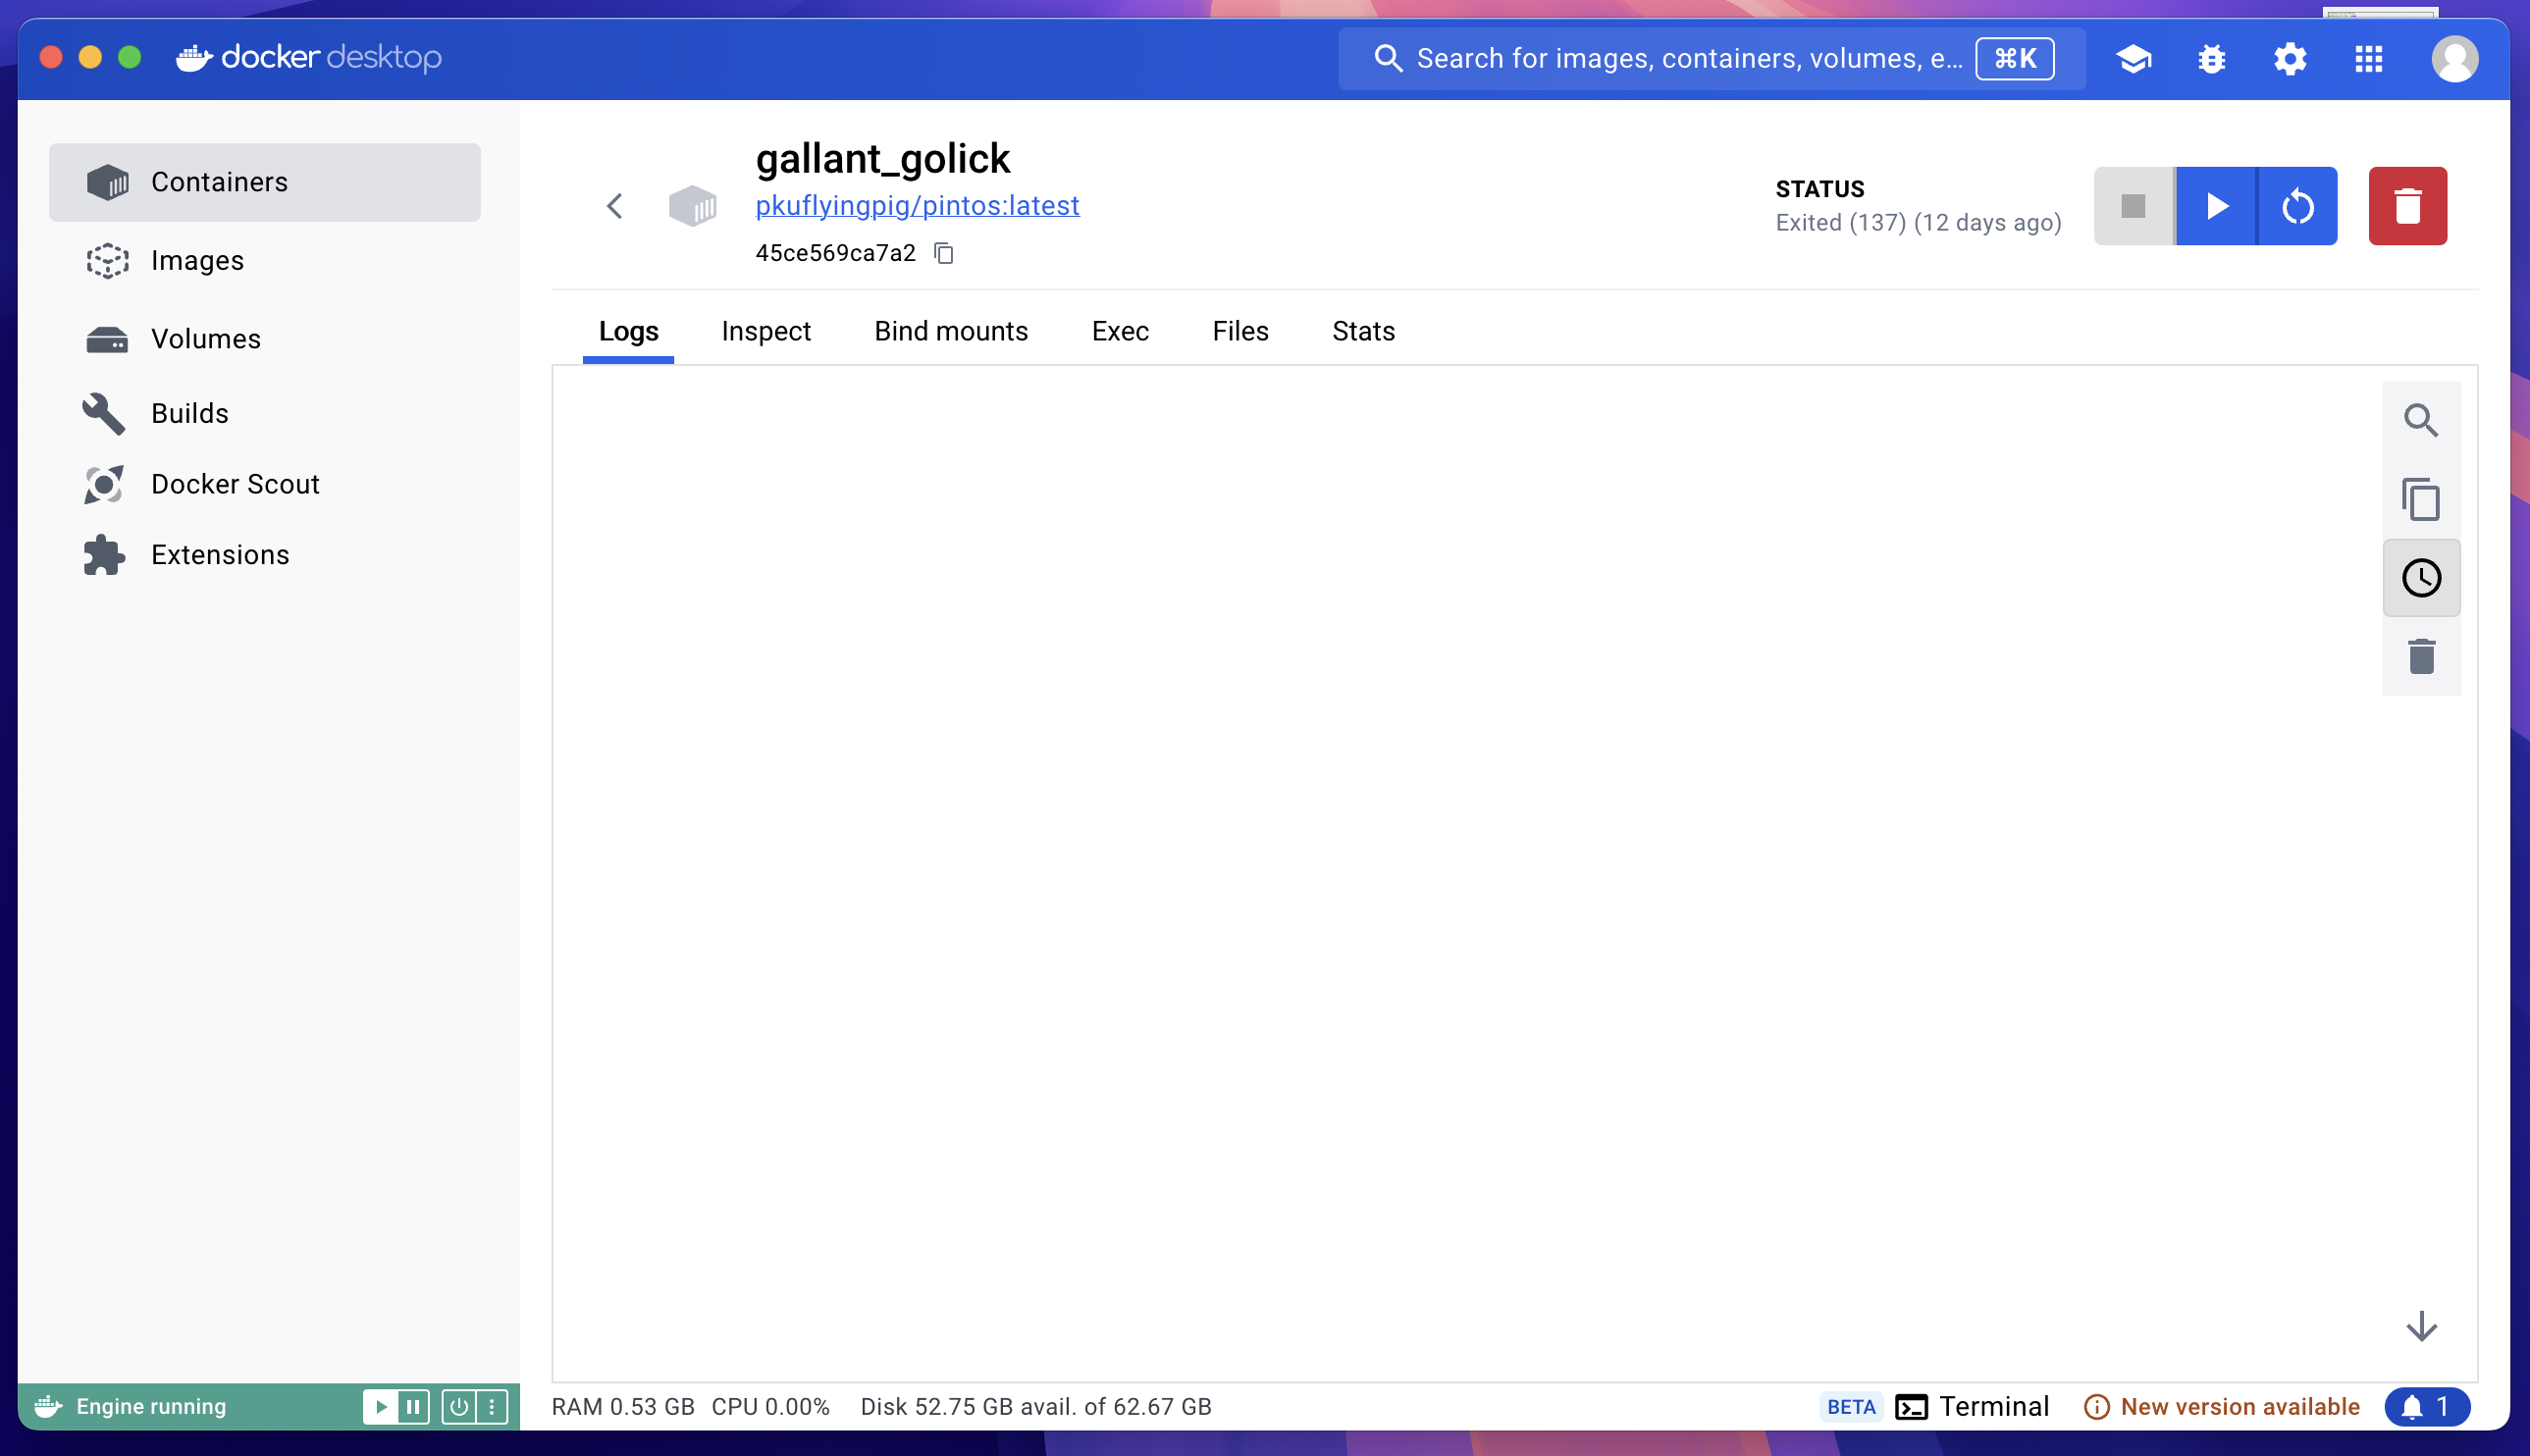
\includegraphics[width=0.9\textwidth]{img/docker_install.png}
	\caption{Docker容器}
\end{figure}

接着使用下面的命令实现磁盘挂载,方便文件管理:

\begin{lstlisting}[language=Bash, title=启动Docker容器并挂载文件]
	docker run -it --rm --name pintos --mount type=bind,\
	source=/Users/wanghaisheng/Desktop/Coding/ECNU-Operating-System-WHS/pintos,\
	target=/home/PKUOS/pintos pkuflyingpig/pintos bash
\end{lstlisting}

完成后如下图所示:

\begin{figure}[H]
	\centering
	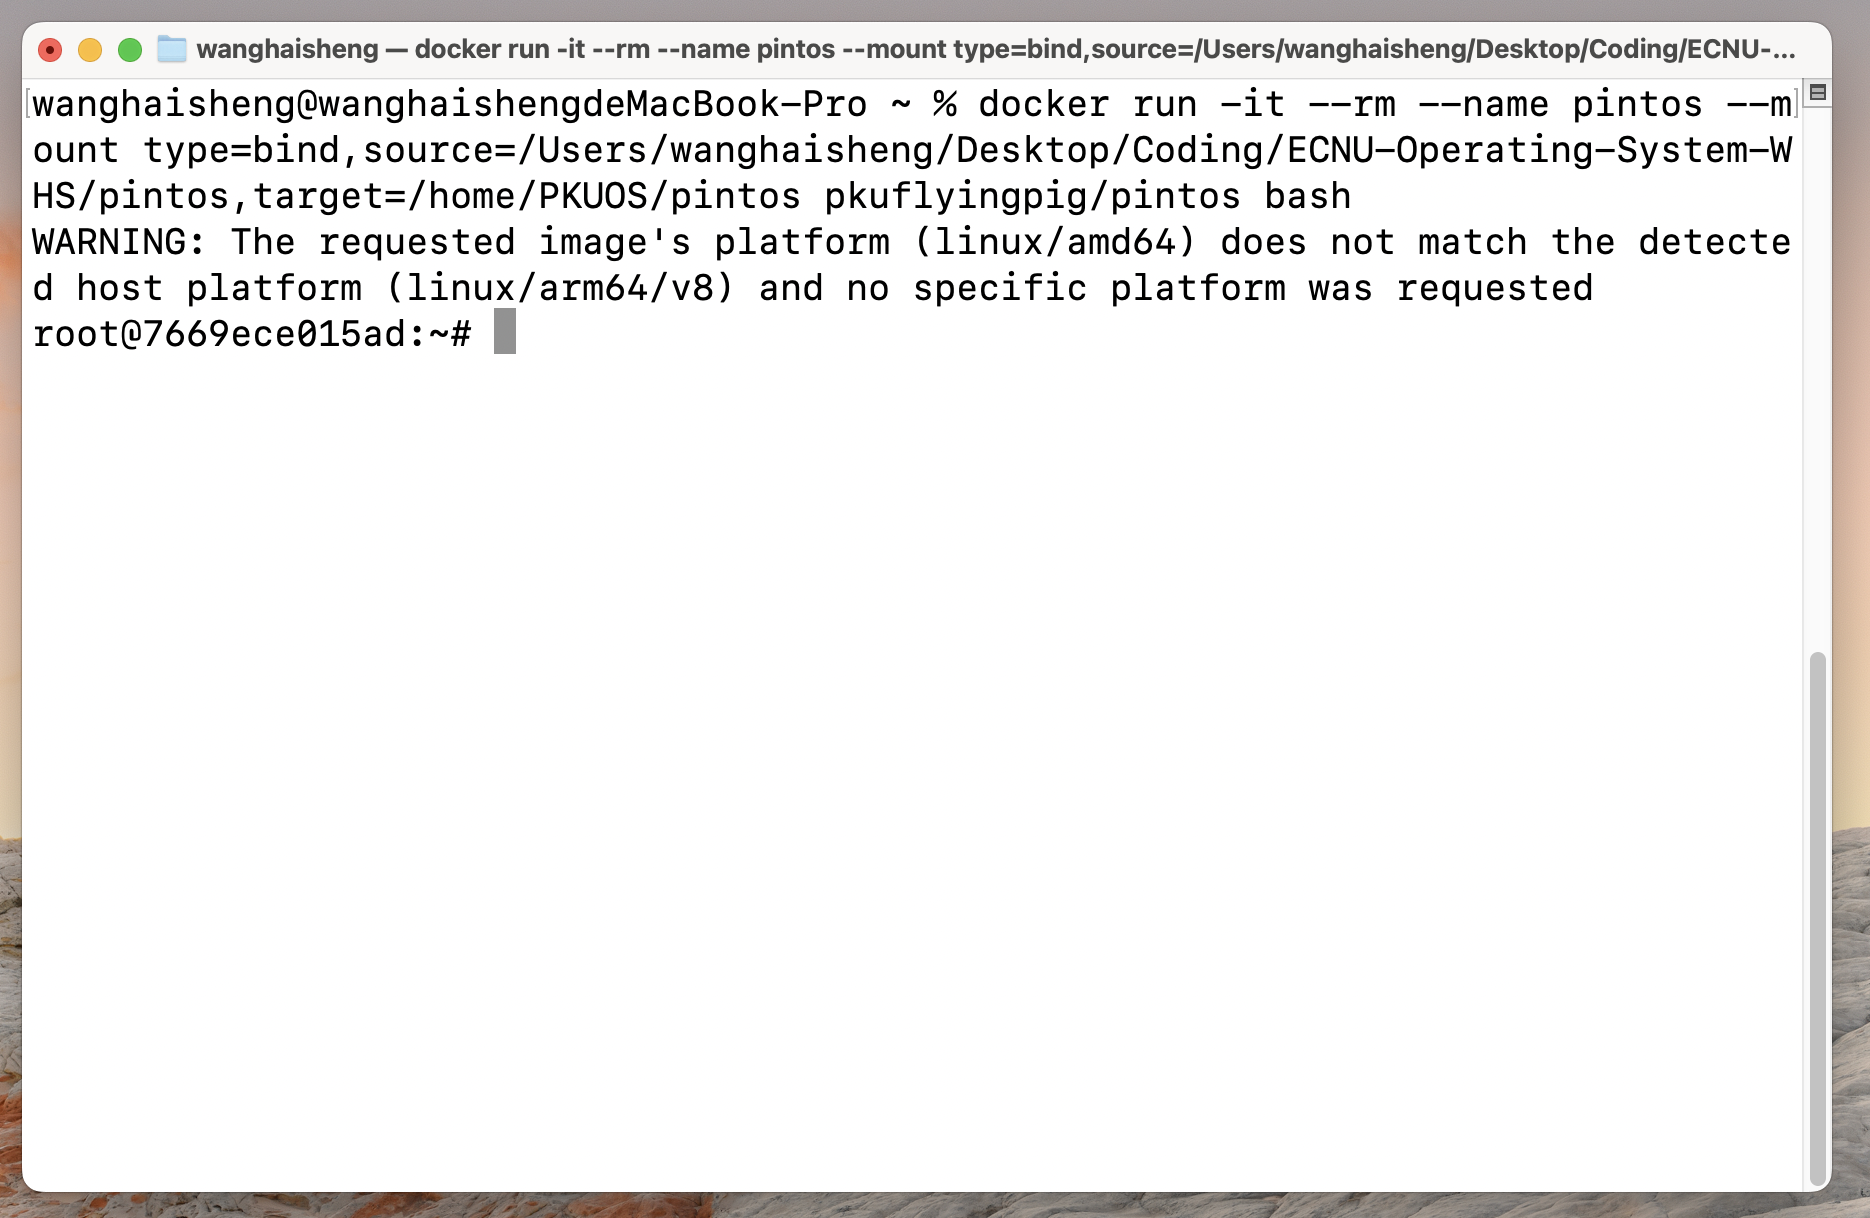
\includegraphics[width=0.9\textwidth]{img/run_docker.png}
	\caption{完成环境配置}
\end{figure}

\normalsize

\section{实验过程}

\subsection{相关源代码分析}

\begin{enumerate}
	\item \textbf{alarm\_priority\_thread}:此文件展示了\texttt{alarm\_priority}相关的线程测试。在PintOS中,\texttt{alarm\_priority}测试用于验证线程的优先级调度机制是否正确实现,确保在唤醒过程中线程按优先级顺序进行唤醒,而不是使用默认的FIFO顺序。
	
	\begin{figure}[H]
		\centering
		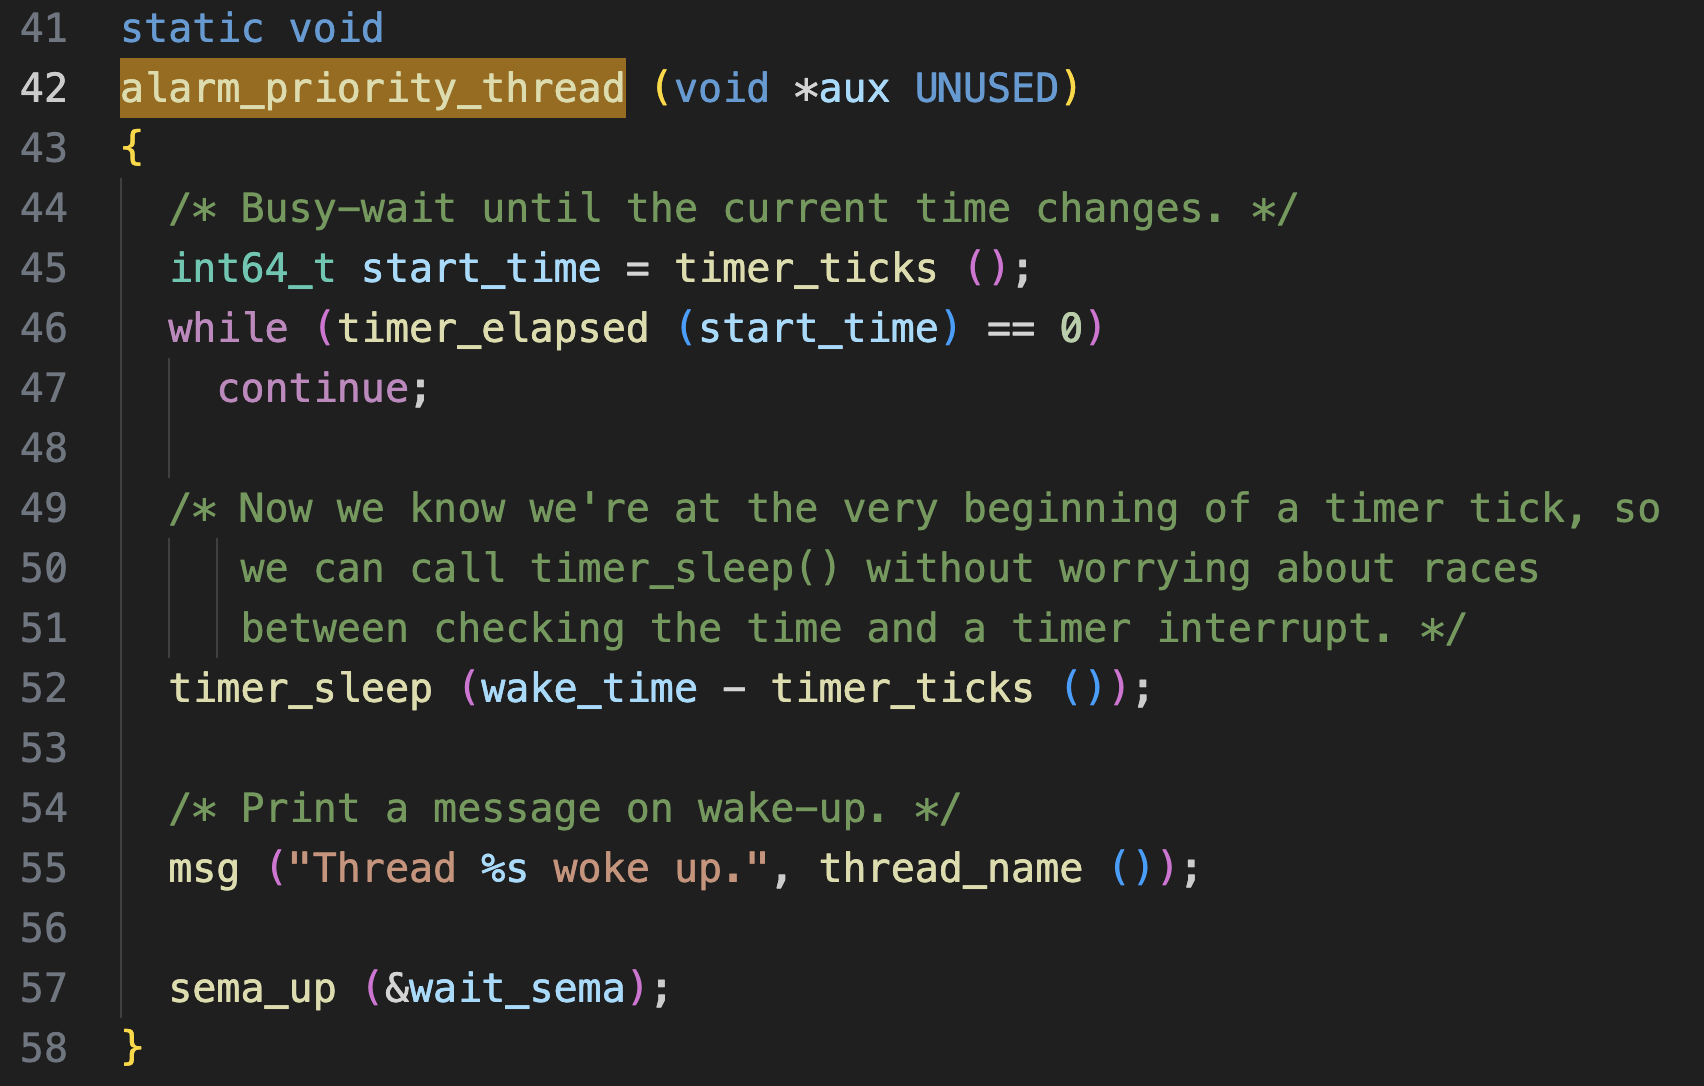
\includegraphics[width=0.6\textwidth]{img/alarm_priority_thread.png}
		\caption{\texttt{alarm\_priority\_thread} 测试的输出结果}
	\end{figure}
	
	\item \textbf{init\_thread}:在PintOS中,\texttt{init\_thread}函数的作用是初始化一个新线程结构体,将其状态设置为阻塞,并为它分配必要的资源,包括栈空间、优先级和线程名。该函数确保新线程在就绪队列中按设定的方式等待调度。
	
	\begin{figure}[H]
		\centering
		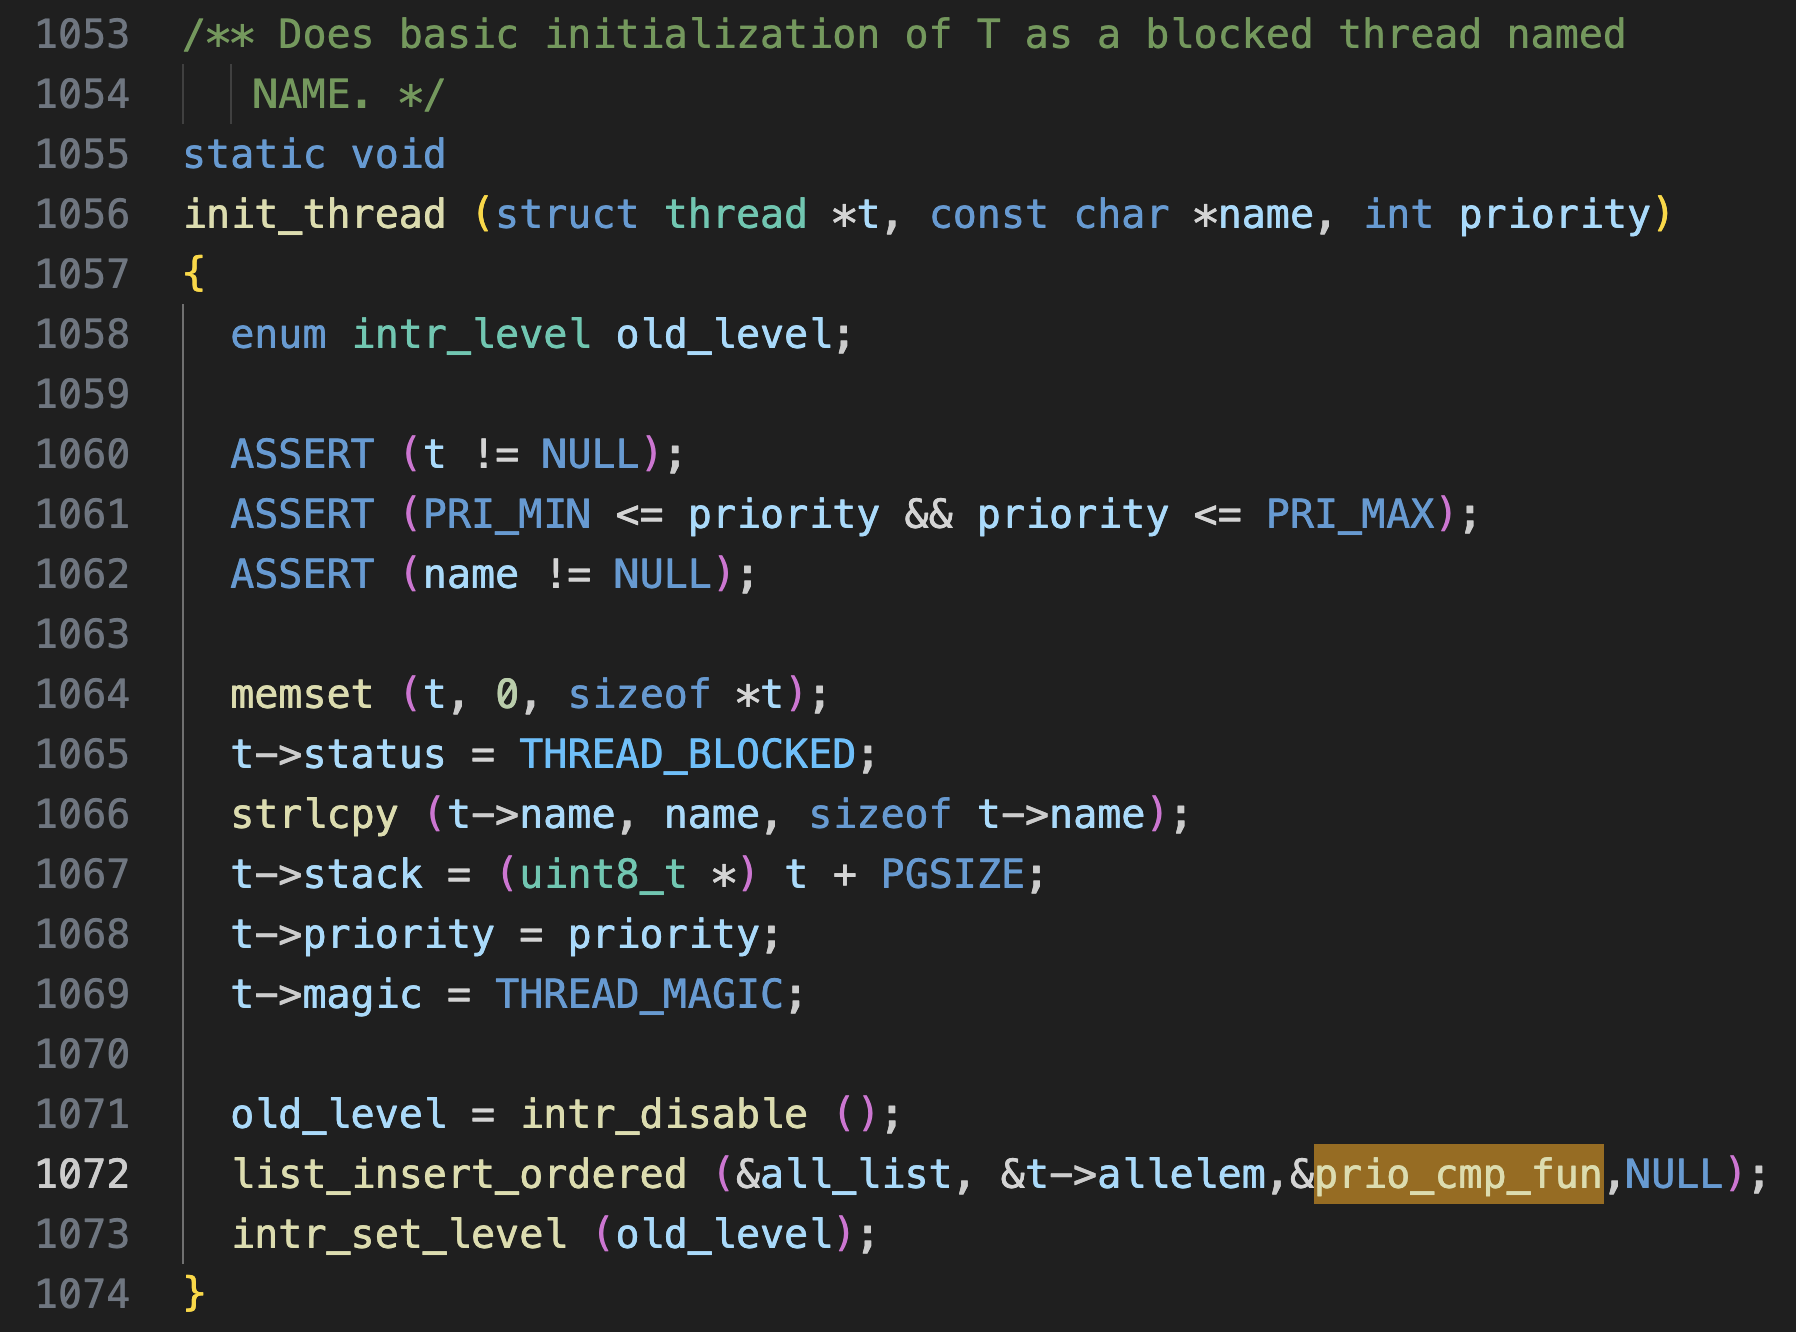
\includegraphics[width=0.6\textwidth]{img/init_thread.png}
		\caption{\texttt{init\_thread}函数实现}
	\end{figure}
	
	\item \textbf{list\_pop\_front}:\texttt{list\_pop\_front}是一个链表操作函数,用于从链表的头部弹出并返回第一个元素。该函数在PintOS中常用于从就绪队列中选择下一个要运行的线程,因为就绪队列中的线程按特定顺序排列,队首元素即为优先级最高的线程。
	
	\begin{figure}[H]
		\centering
		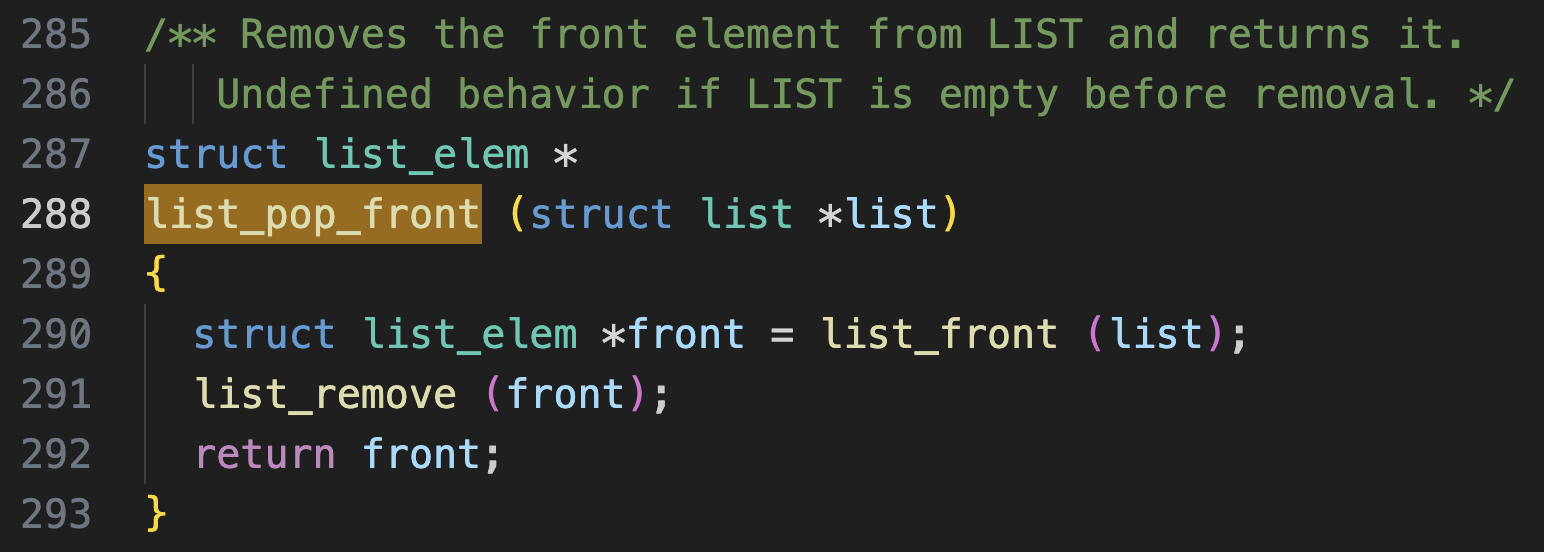
\includegraphics[width=0.6\textwidth]{img/list_pop_front.png}
		\caption{\texttt{list\_pop\_front}函数实现}
	\end{figure}
	
	\item \textbf{list\_push\_back}:\texttt{list\_push\_back}是另一个链表操作函数,用于将一个元素插入到链表的末尾。在PintOS默认的调度中,该函数用于将新线程插入到就绪队列的尾部,符合FIFO调度机制。不过在优先级调度模式中,\texttt{list\_push\_back}会被\texttt{list\_insert\_ordered}替代,以实现按优先级顺序插入。
	
	\begin{figure}[H]
		\centering
		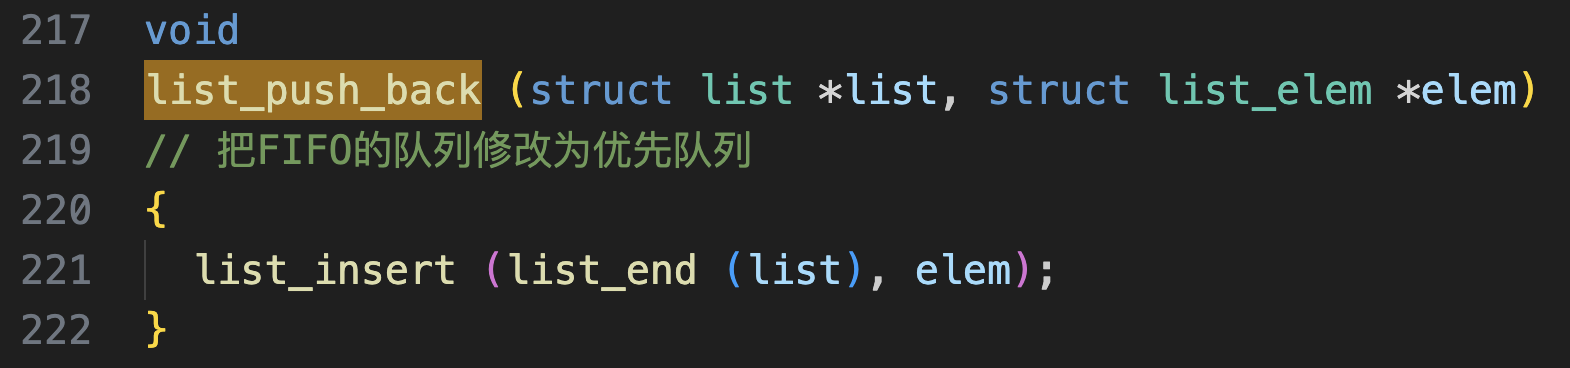
\includegraphics[width=0.6\textwidth]{img/list_push_back.png}
		\caption{\texttt{list\_push\_back}函数实现}
	\end{figure}
	
	\item \textbf{next\_thread\_to\_run}:\texttt{next\_thread\_to\_run}函数的作用是从就绪队列中选择下一个要运行的线程。默认情况下,它会选择队首的线程并将其返回。在优先级调度模式下,只要确保就绪队列按优先级排好队,该函数就会直接选择优先级最高的线程。
	
	\begin{figure}[H]
		\centering
		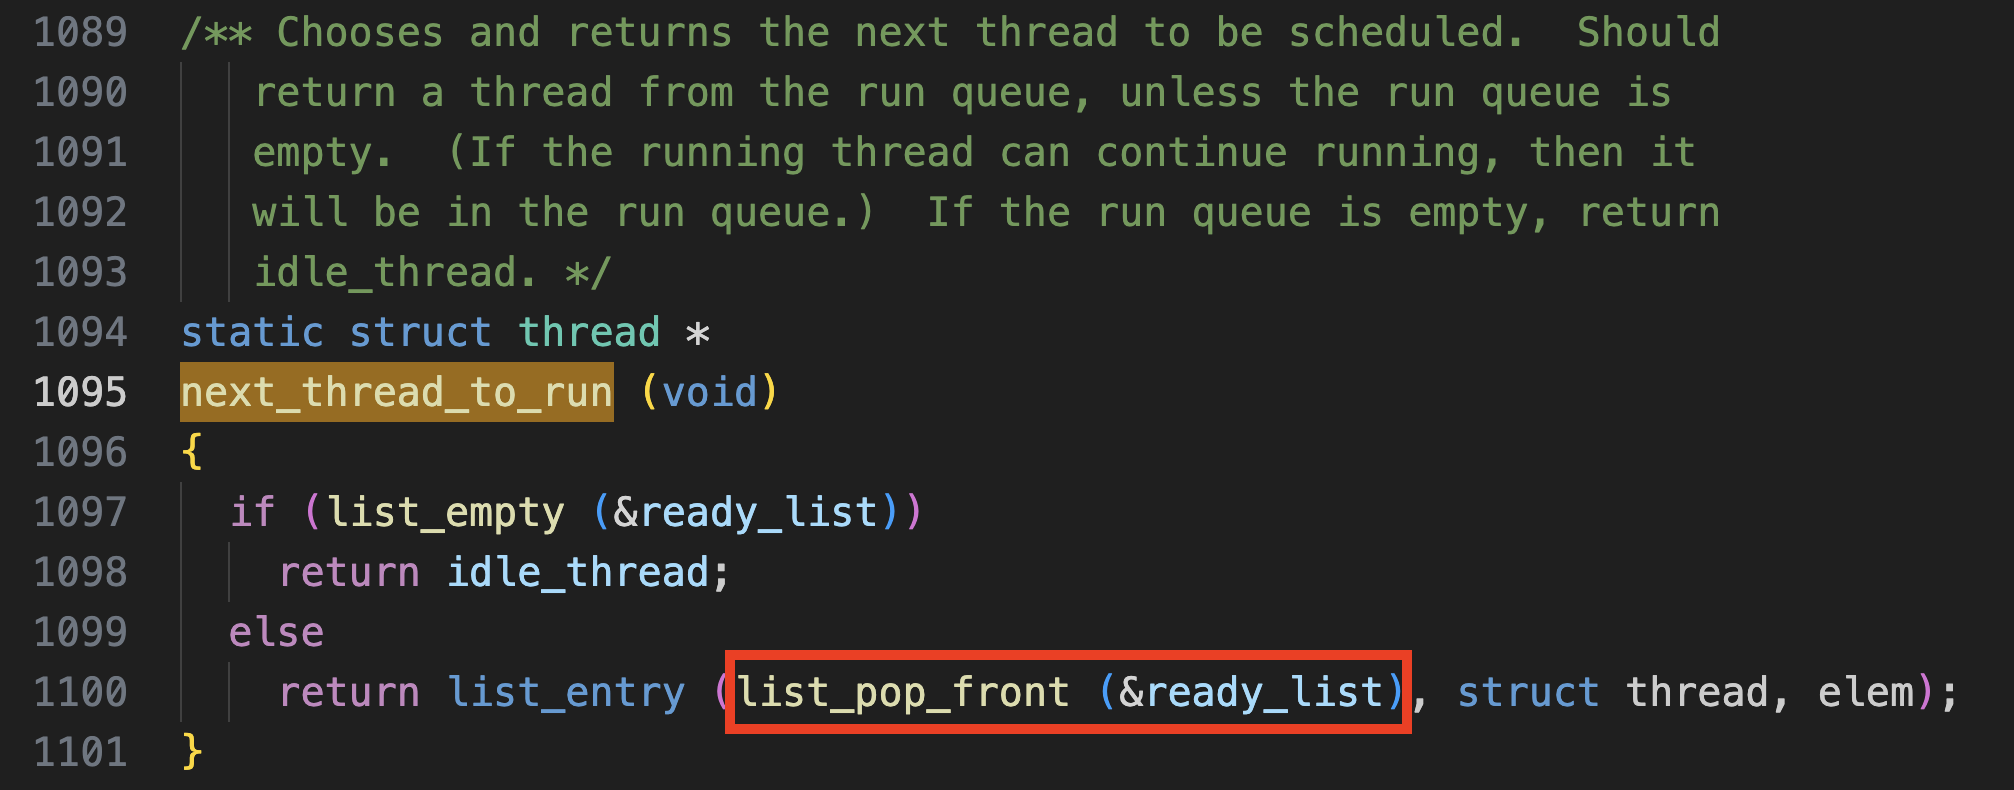
\includegraphics[width=0.6\textwidth]{img/next_thread_to_run.png}
		\caption{\texttt{next\_thread\_to\_run}函数实现}
	\end{figure}
	
	\item \textbf{prio\_cmp\_fun}:这是用户自定义的优先级比较函数,用于在\texttt{list\_insert\_ordered}函数中作为参数,以保证线程根据优先级顺序插入到就绪队列中。该函数比较两个线程的优先级并返回布尔值,确保高优先级的线程被插入到队列的更前方。
	
	\begin{figure}[H]
		\centering
		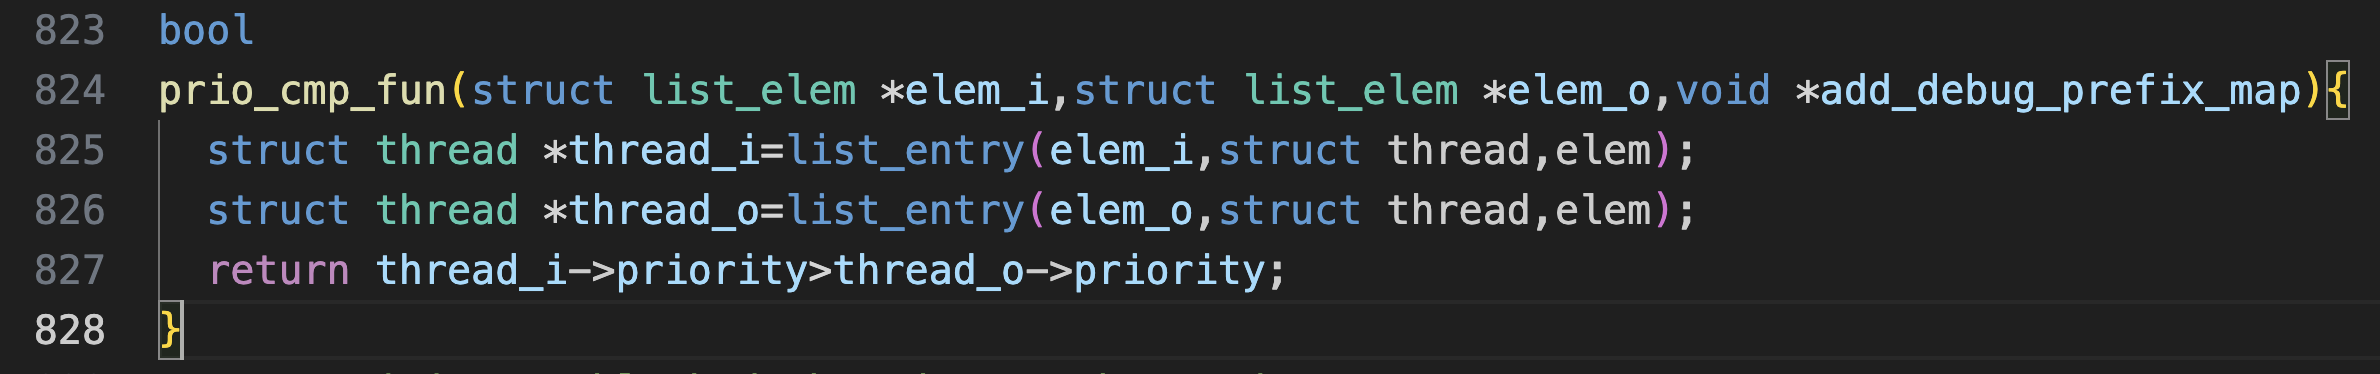
\includegraphics[width=0.6\textwidth]{img/prio_cmp_fun.png}
		\caption{\texttt{prio\_cmp\_fun}函数实现}
	\end{figure}
	
	\item \textbf{test\_alarm\_priority}:这是\texttt{alarm\_priority}测试的实现,用于验证线程在休眠结束后按优先级顺序唤醒。该测试确保线程调度正确执行优先级调度,即唤醒线程时从高到低的顺序运行,而不是随意顺序或FIFO顺序。
	
	\begin{figure}[H]
		\centering
		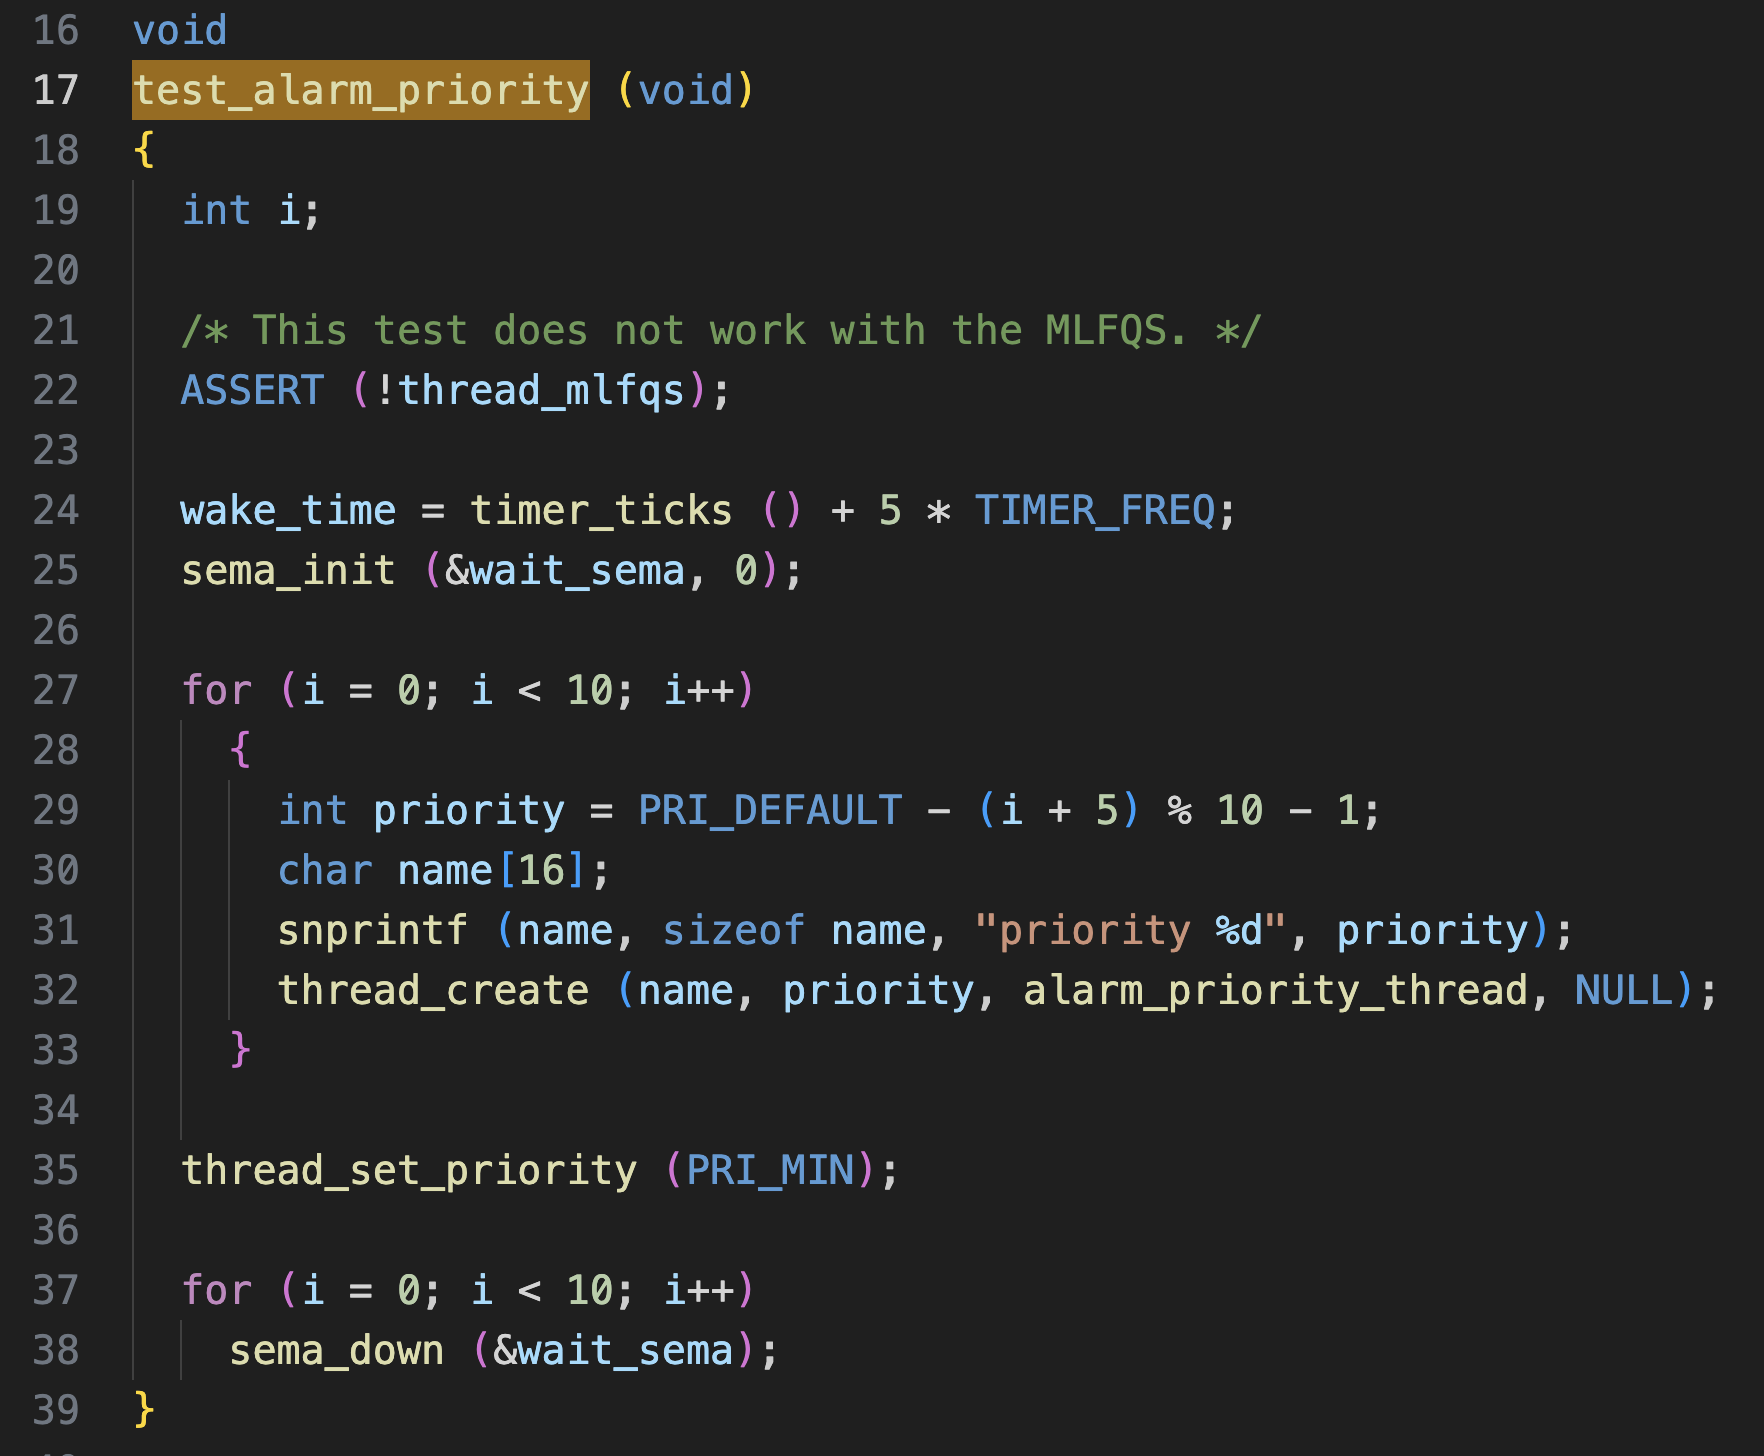
\includegraphics[width=0.6\textwidth]{img/test_alarm_priority.png}
		\caption{\texttt{test\_alarm\_priority}测试实现}
	\end{figure}
	
	\item \textbf{thread\_unblock}:\texttt{thread\_unblock}函数在PintOS中用于将阻塞状态的线程变为就绪状态。它通常会将线程插入到就绪队列中。默认情况下,使用的是\texttt{list\_push\_back}插入,但在优先级调度实现中,会用到\texttt{list\_insert\_ordered}函数,以确保按优先级顺序排列。
	
	\begin{figure}[H]
		\centering
		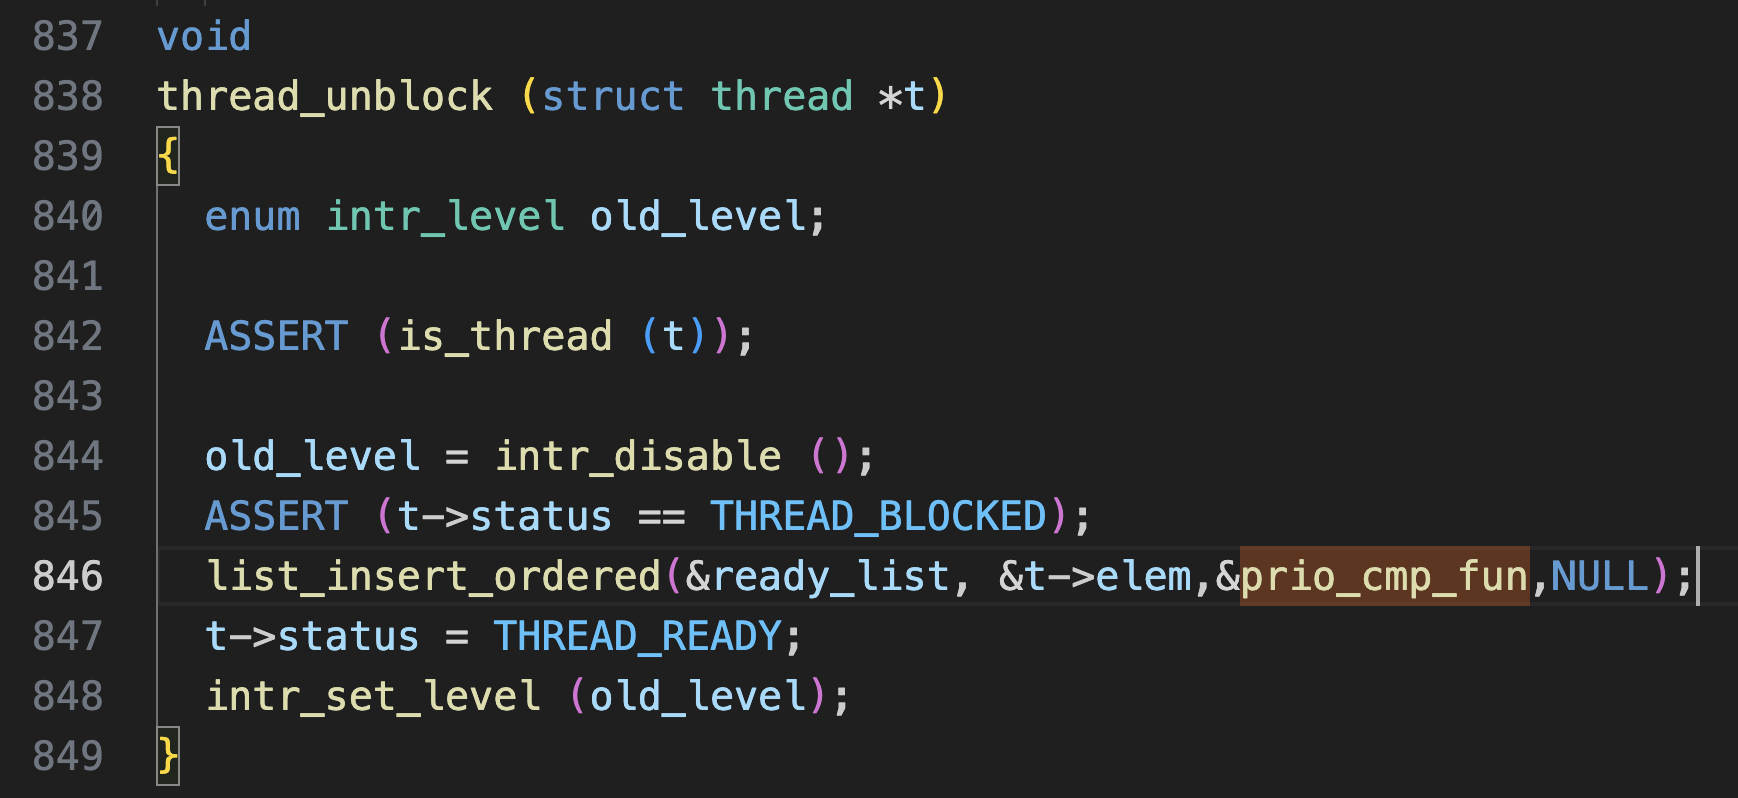
\includegraphics[width=0.6\textwidth]{img/thread_unblock.png}
		\caption{\texttt{thread\_unblock}函数实现}
	\end{figure}
	
	\item \textbf{thread\_yield}:\texttt{thread\_yield}函数用于当前线程主动放弃CPU时间,将自身状态设为就绪,并将其重新插入到就绪队列中。这通常用于实现抢占式调度,例如当有高优先级线程到来时,低优先级线程需要让出CPU资源。
	
	\begin{figure}[H]
		\centering
		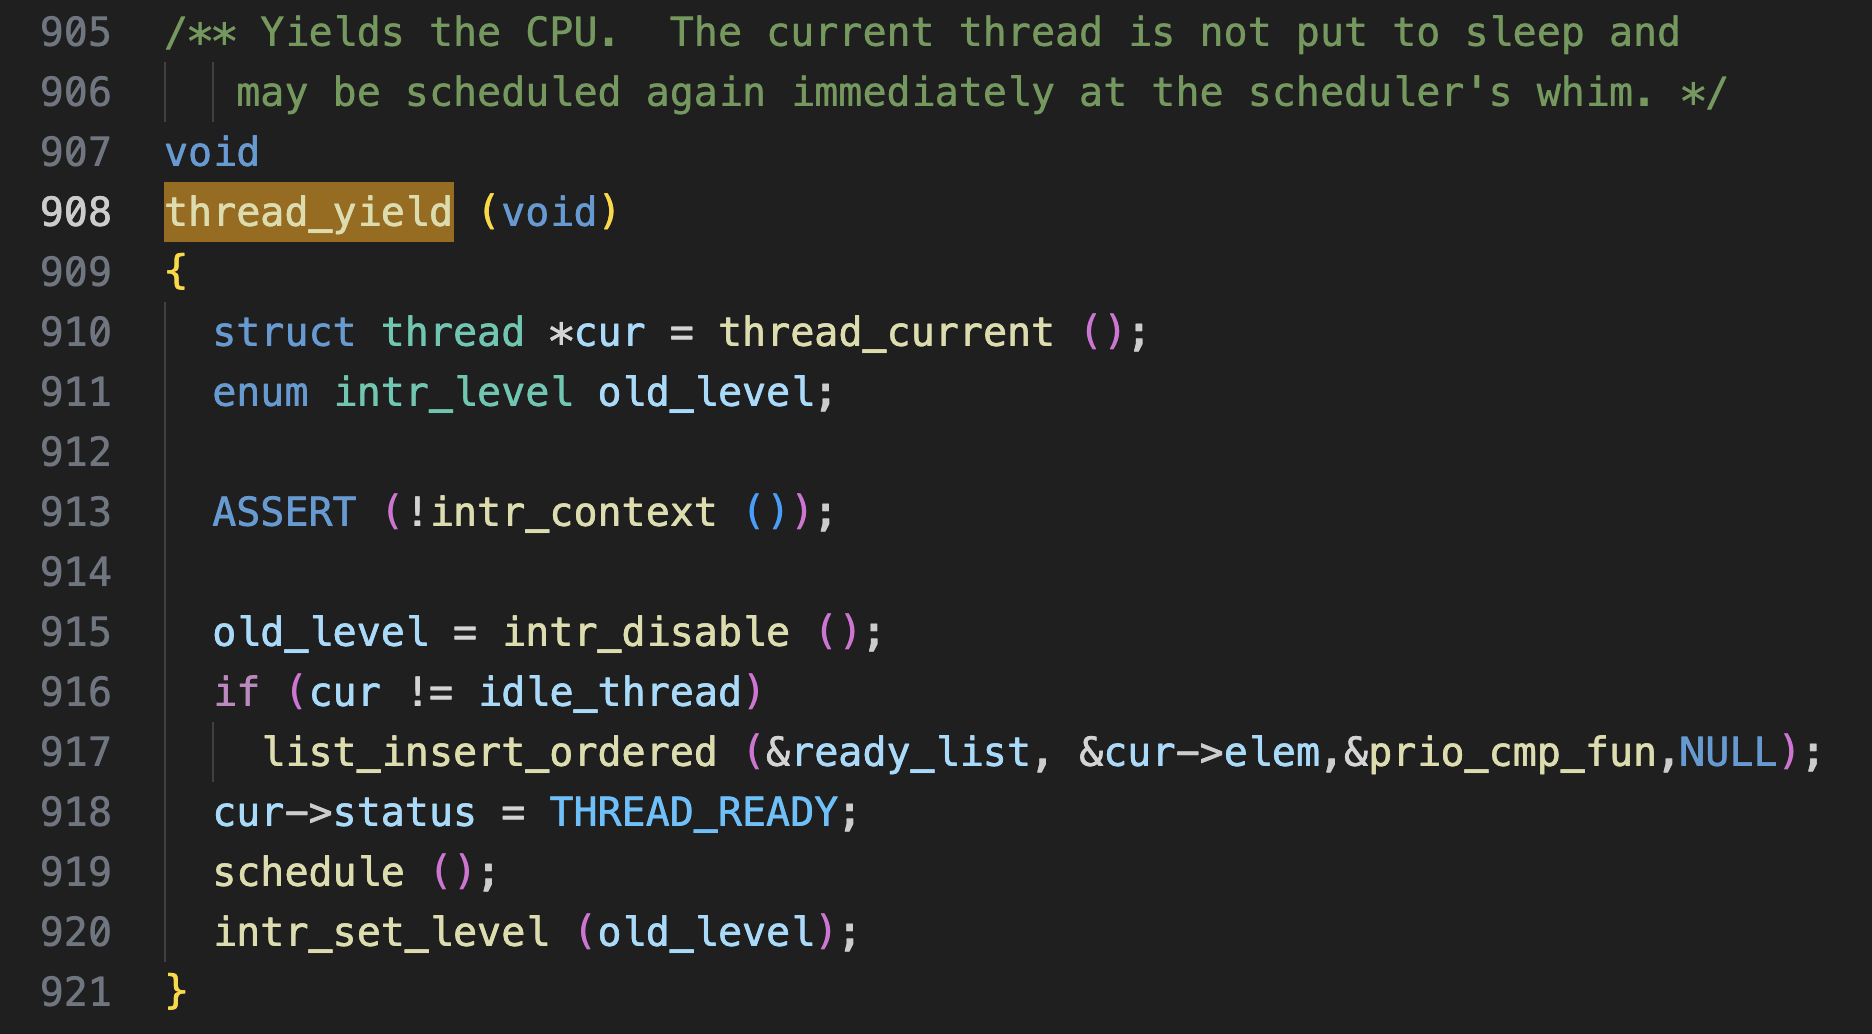
\includegraphics[width=0.6\textwidth]{img/thread_yield.png}
		\caption{\texttt{thread\_yield}函数实现}
	\end{figure}
	
	\item \textbf{threadh}:这个文件名对应\texttt{thread.h},这是PintOS中定义线程结构和相关函数的头文件。该文件包含线程的各种状态、优先级以及调度相关的函数声明,是PintOS线程管理的核心定义文件之一。
	
	\begin{figure}[H]
		\centering
		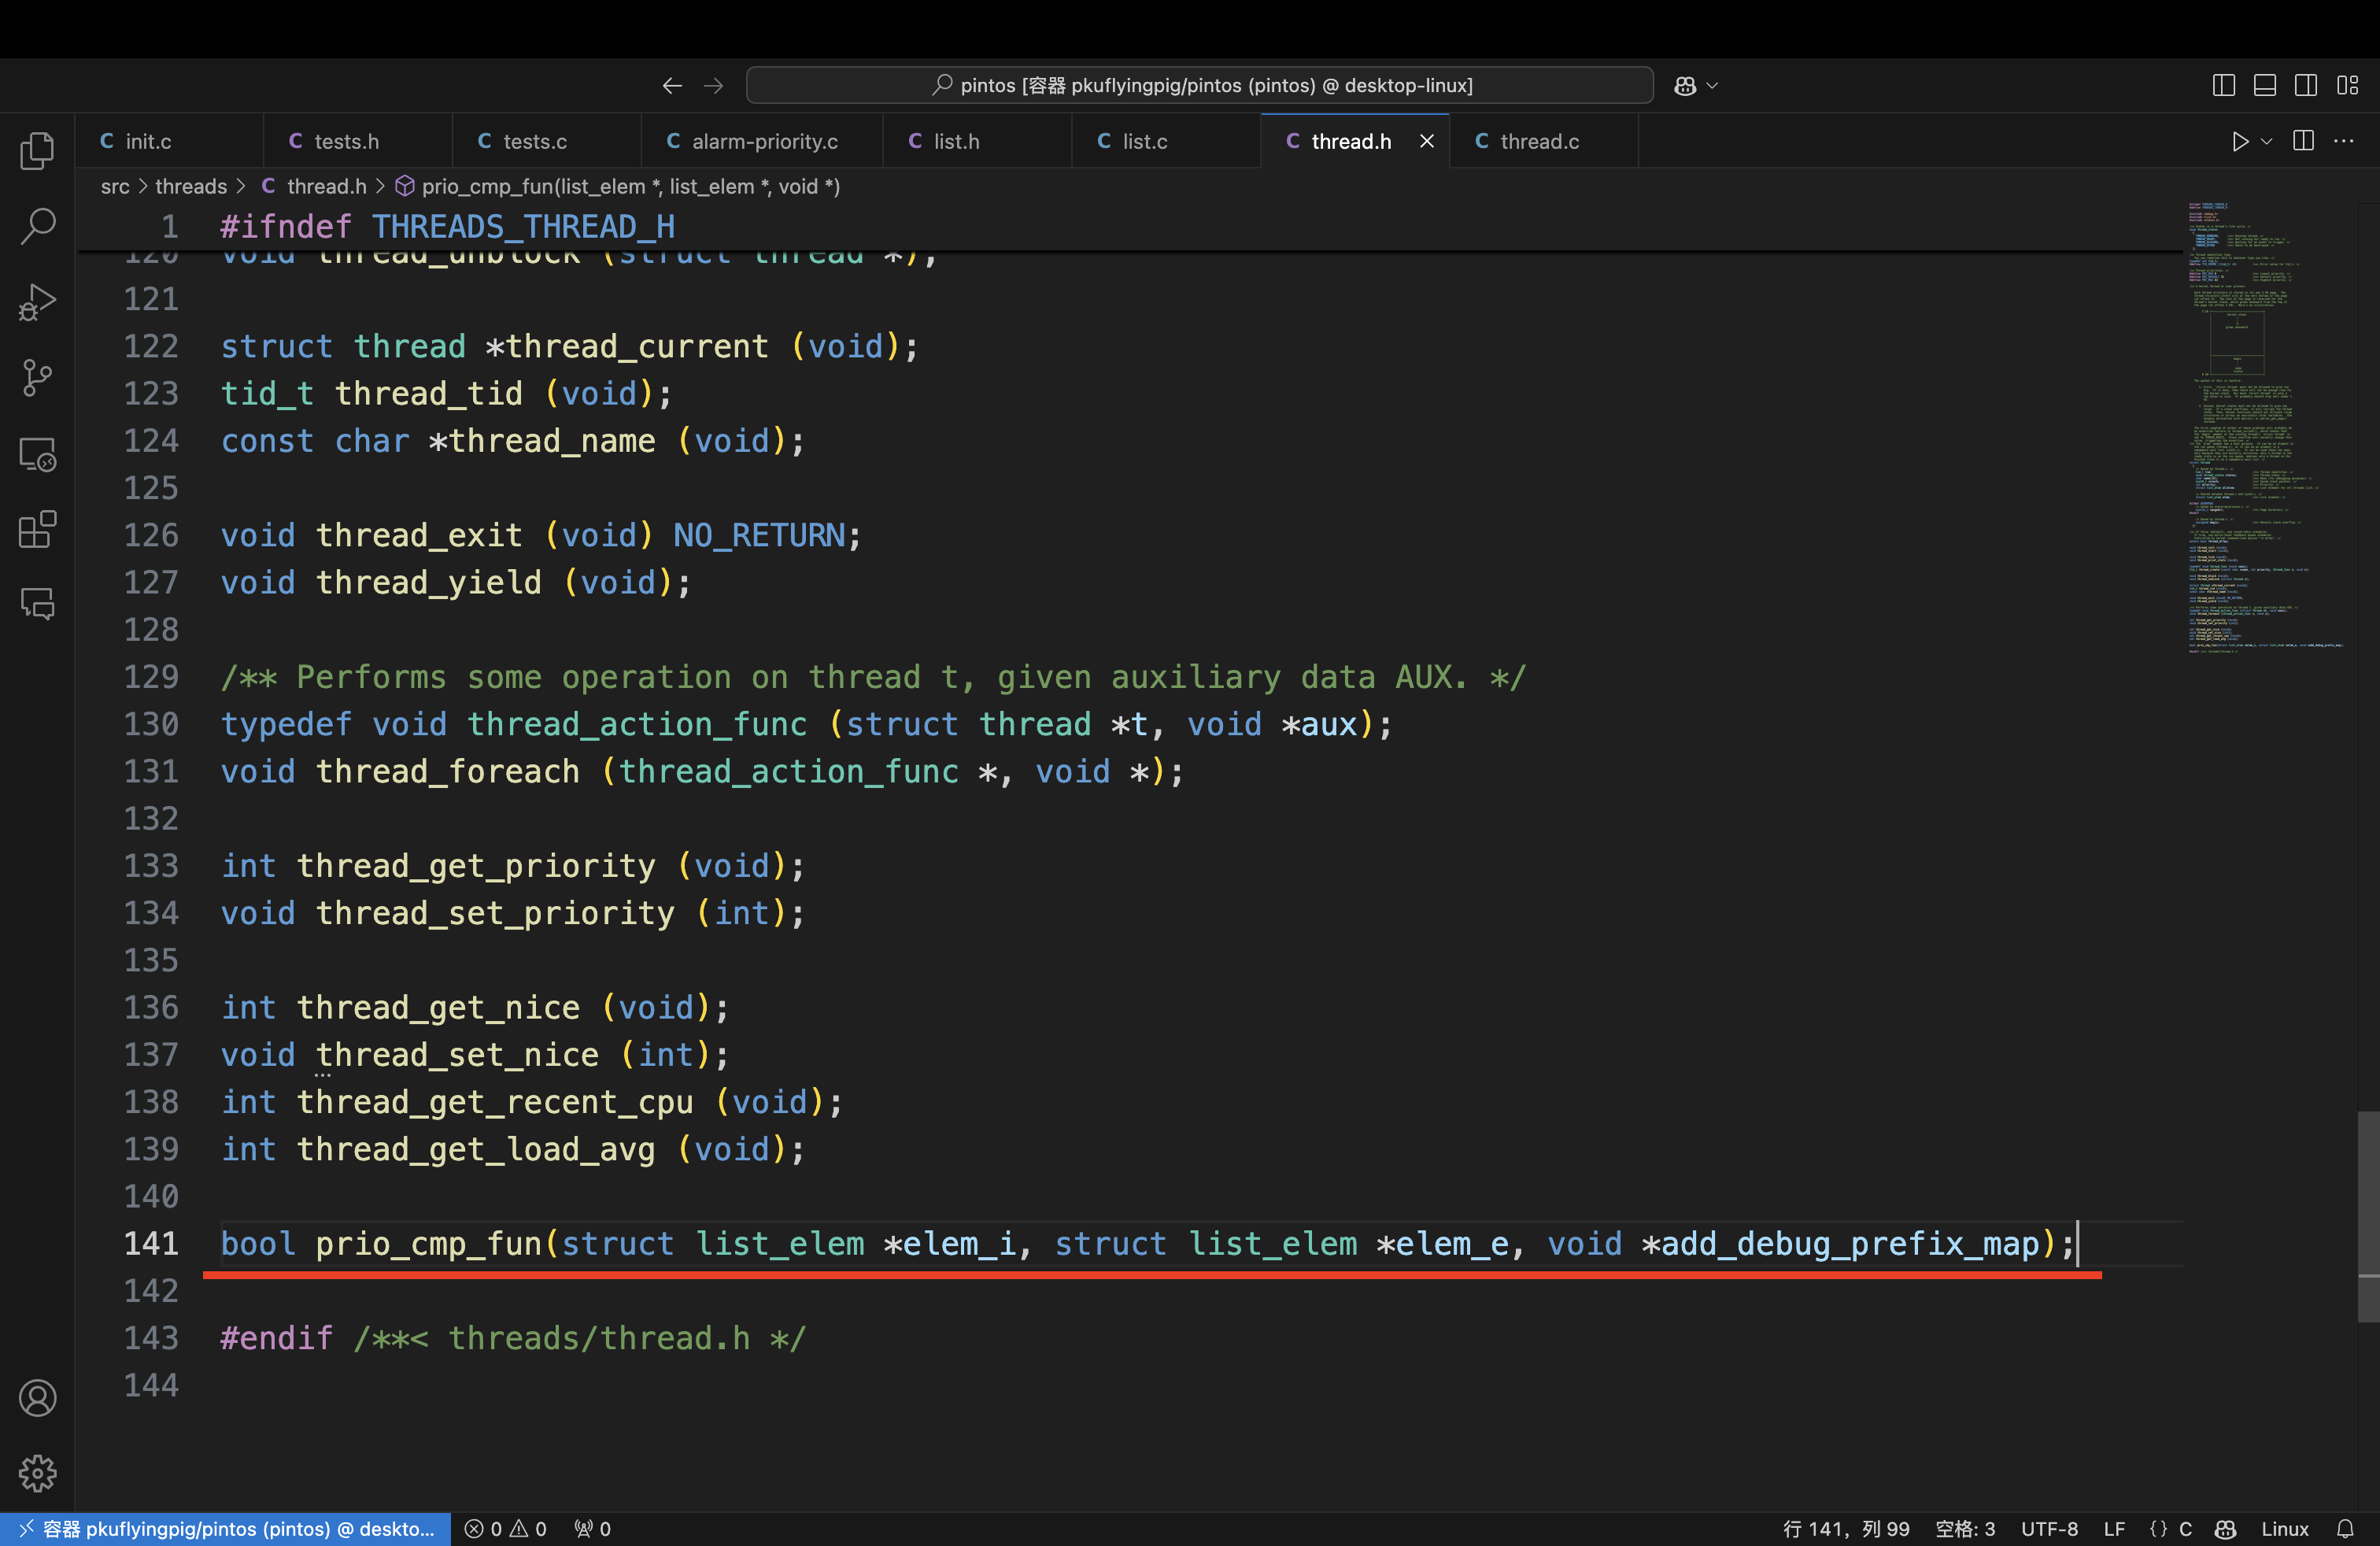
\includegraphics[width=0.6\textwidth]{img/threadh.png}
		\caption{\texttt{thread.h}头文件}
	\end{figure}
\end{enumerate}

\subsection{实现优先级调度}

实验开始前,测试运行结果如下图:

\begin{figure}[H]
	\centering
	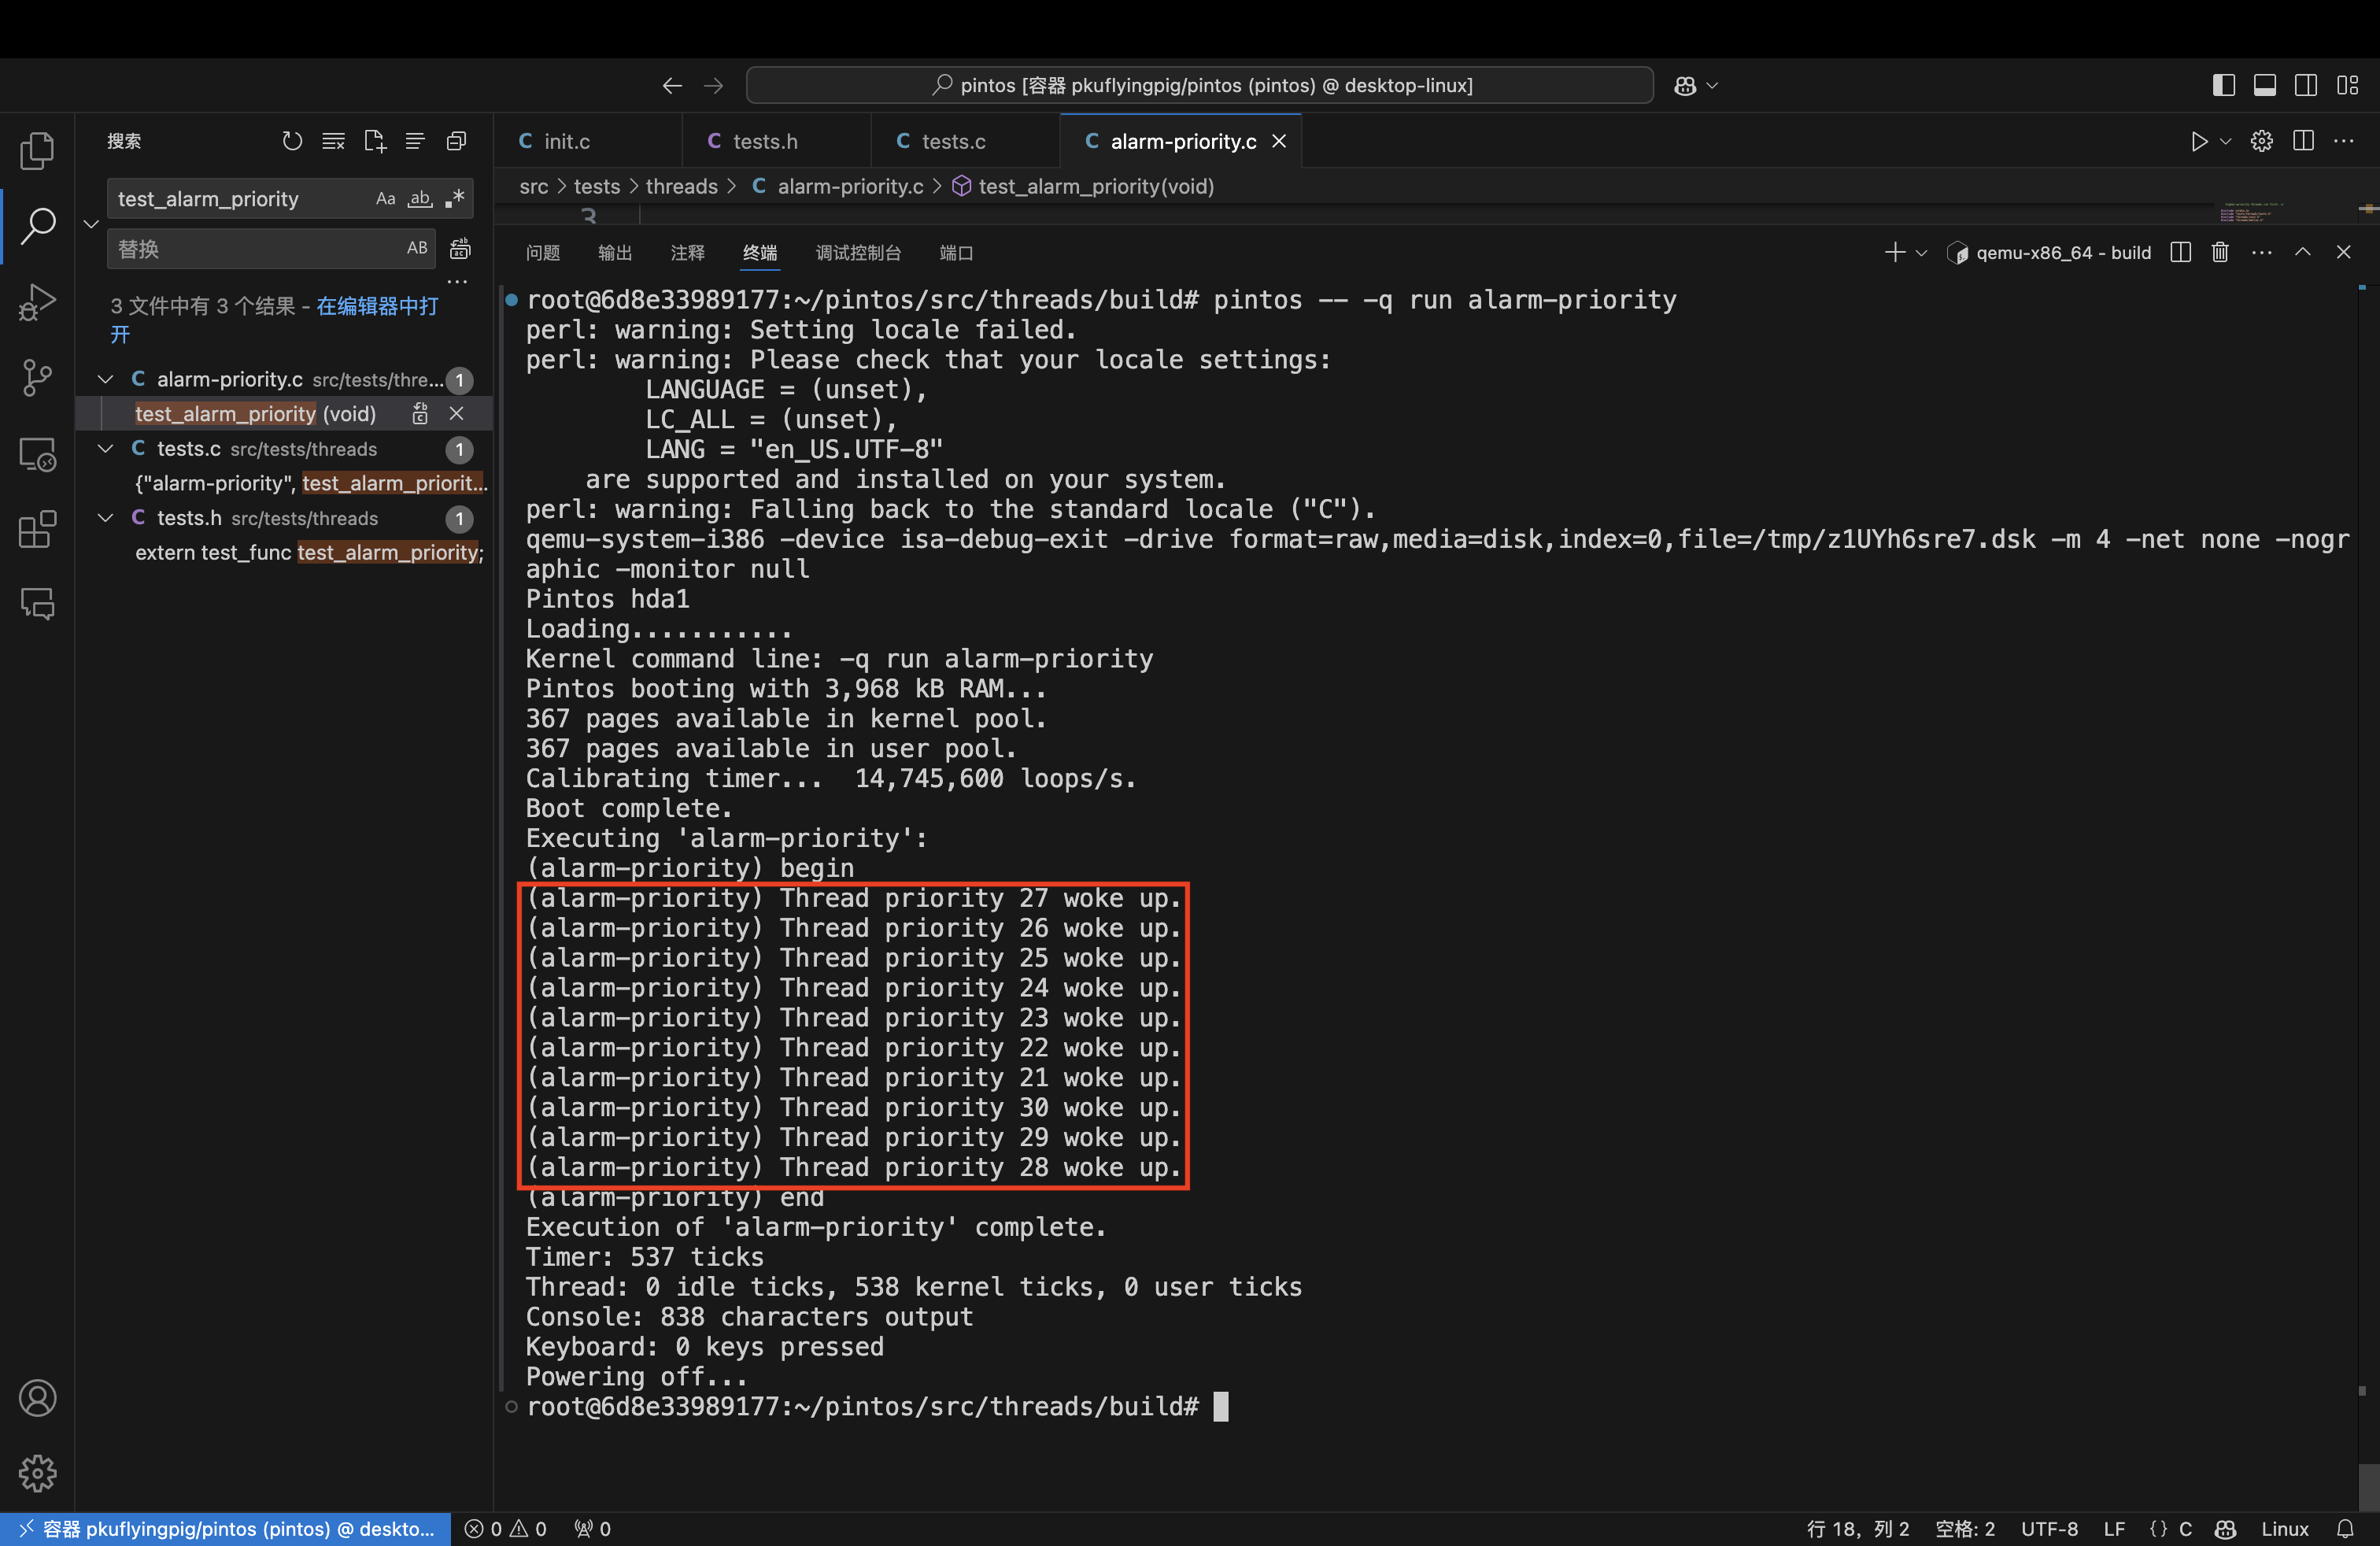
\includegraphics[width=0.9\textwidth]{img/run_origin.png}
	\caption{实验之前的测试结果}
\end{figure}

实验过程中,我采取了以下步骤:

\begin{enumerate}
	\item \textbf{初步测试}:在未修改代码的情况下执行\texttt{make check},观察Pintos的默认调度机制。系统会按照先进先出(FIFO)的顺序调度线程,即按照线程创建的先后顺序执行。通过这一测试,我确认了系统当前的调度机制,并验证了默认实现不符合优先级调度的预期目标,因此测试未通过。
	
	\item \textbf{编写优先级比较函数}:在\texttt{thread.c}文件中添加自定义优先级比较函数\texttt{bool prio\_cmp\_fun()}。该函数用于比较两个线程的优先级,以此决定线程在就绪队列中的插入位置。代码如下:
	
	\begin{lstlisting}[language=C, basicstyle=\ttfamily, keywordstyle=\color{blue}]
bool prio_cmp_fun(struct list_elem *elem_i, struct list_elem *elem_o, void *aux) {
	struct thread *thread_i = list_entry(elem_i, struct thread, elem);
	struct thread *thread_o = list_entry(elem_o, struct thread, elem);
	return thread_i->priority > thread_o->priority;
}
	\end{lstlisting}
	
	该函数通过使用\texttt{list\_entry}宏来访问线程结构体,将每个线程的优先级进行比较,并返回布尔值。返回值为真表示\texttt{thread\_i}优先级高于\texttt{thread\_o},从而确保线程按优先级高低依次排在就绪队列的前方。
	
	\item \textbf{替换插入方法}:为了使就绪队列按优先级顺序排序,将\texttt{thread\_unblock}和\texttt{thread\_yield}函数中的默认插入函数\texttt{list\_push\_back}替换为\texttt{list\_insert\_ordered},并将前面定义的\texttt{prio\_cmp\_fun}作为参数传入。这样,线程在被插入到就绪队列时会按照优先级顺序排列。
	
	\item \textbf{调试与解决错误}:首次运行修改后的代码时,系统报缺少参数错误。经过仔细检查和咨询助教,发现调用\texttt{list\_insert\_ordered}时需提供两个额外参数:优先级比较函数指针\texttt{\&prio\_cmp\_fun}和辅助参数\texttt{NULL}。在补充这两个参数后,代码成功运行。
	
	\item \textbf{编译与测试}:在完成上述修改后,重新执行\texttt{make check}命令进行编译和测试,观察到\texttt{alarm-priority}测试通过,结果中线程按优先级顺序倒序唤醒,符合预期的优先级调度输出。
\end{enumerate}

实验完成后,单项测试结果如下图:

\begin{figure}[H]
	\centering
	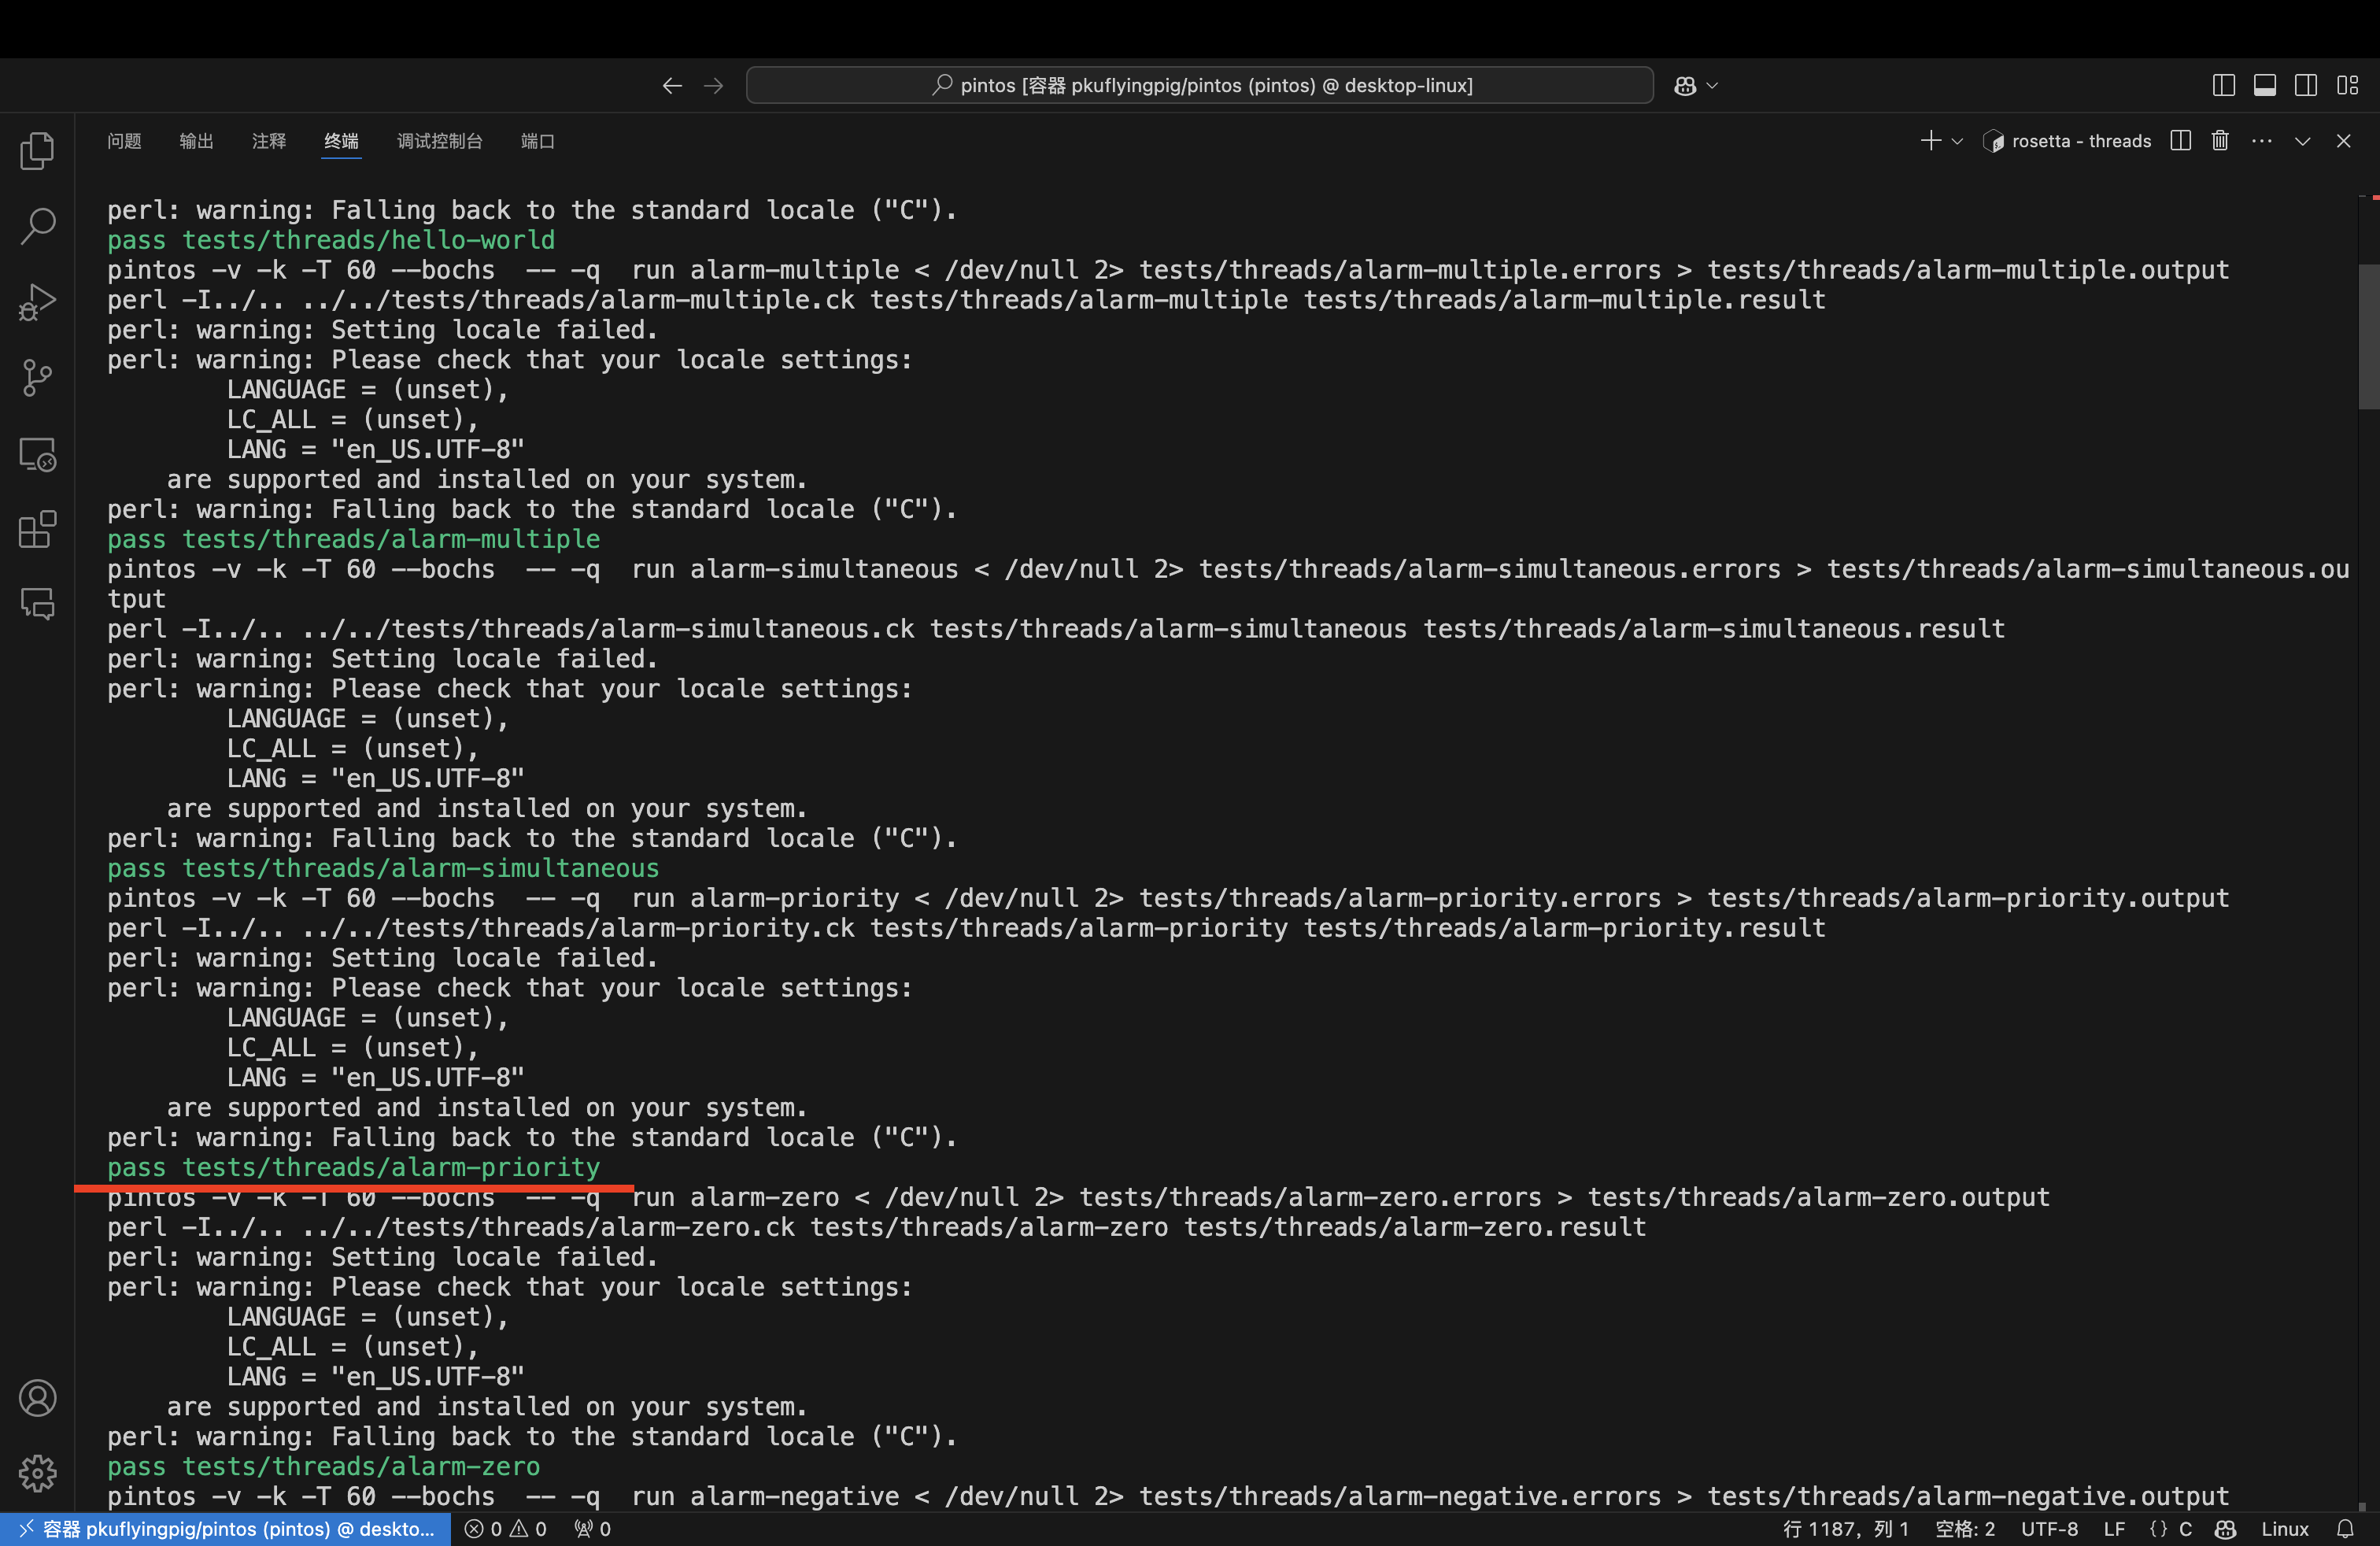
\includegraphics[width=0.9\textwidth]{img/pass.png}
	\caption{单项测试结果}
\end{figure}

总测试结果如下图:

\begin{figure}[H]
	\centering
	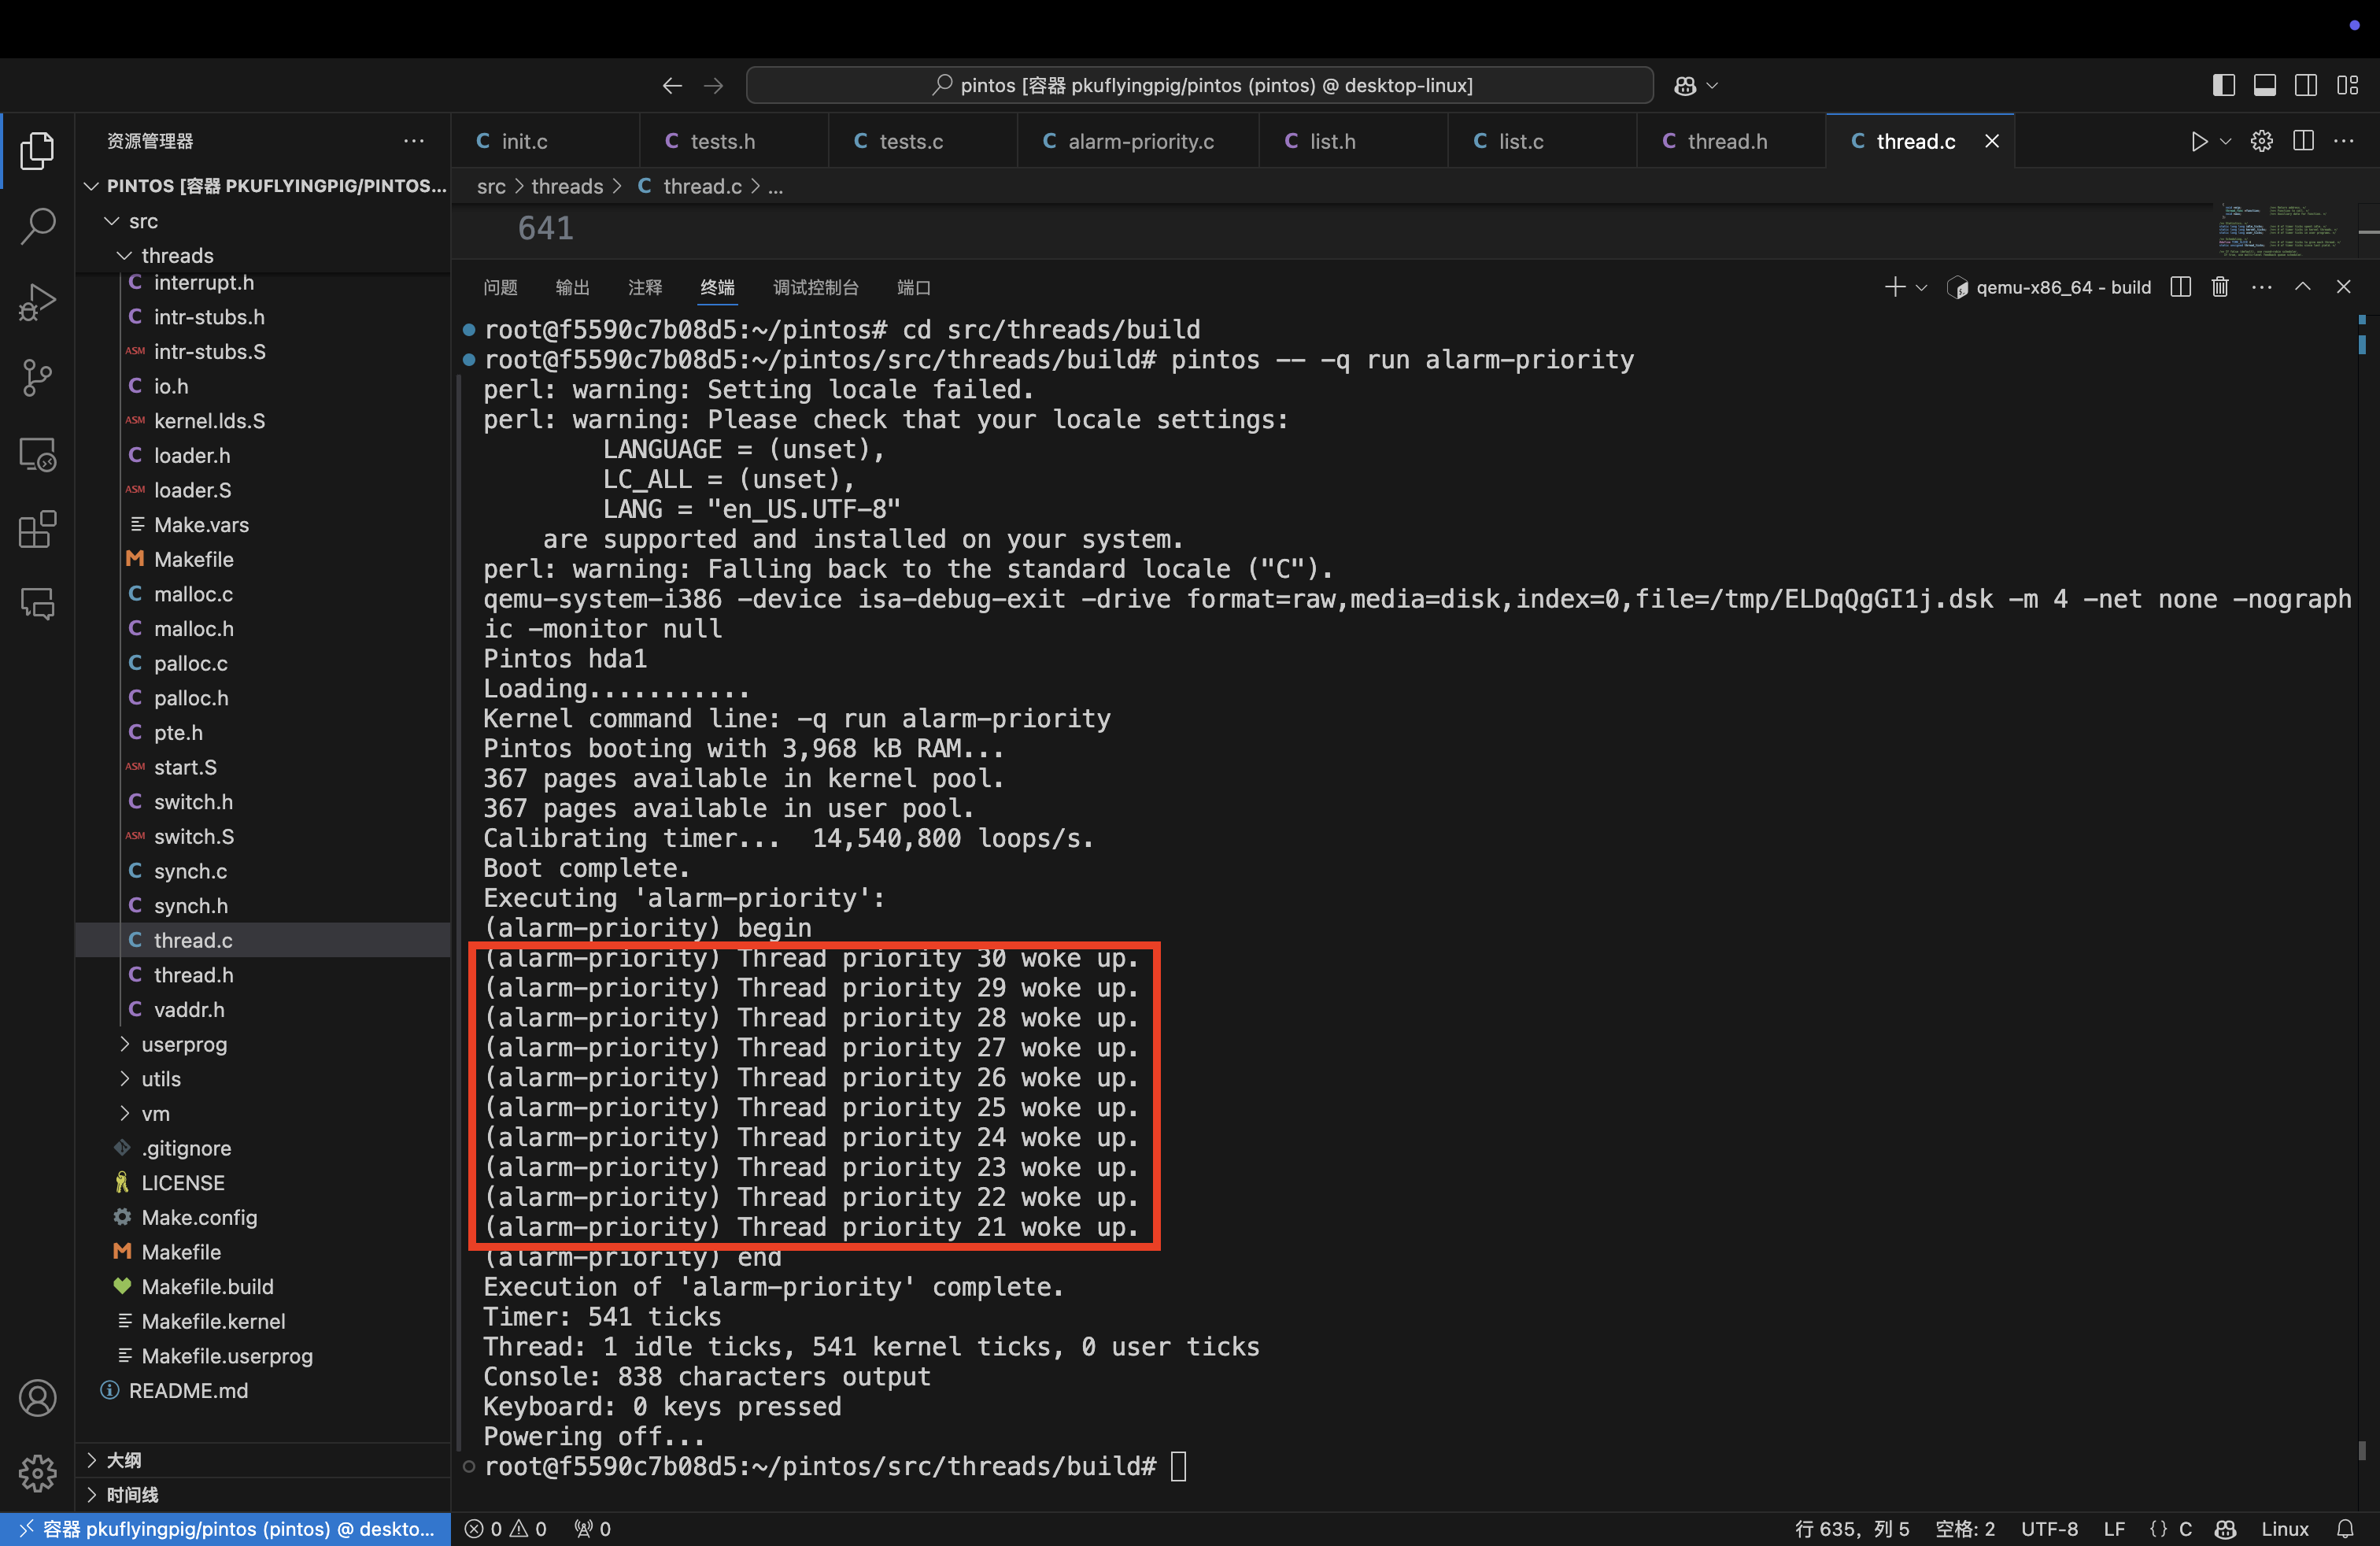
\includegraphics[width=0.9\textwidth]{img/run_final.png}
	\caption{总测试结果}
\end{figure}

实验结果表明,修改后的代码成功实现了优先级调度,测试结果中的线程按优先级倒序唤醒,符合预期输出。

\normalsize

\section{实验总结}

本次实验成功实现了Pintos的优先级调度功能,主要收获包括:

\begin{itemize}
	\item \textbf{掌握了优先级调度的实现方法}:通过自定义比较函数和修改线程插入方式,实现了优先级调度,使得高优先级线程在就绪队列中处于优先位置。
	\item \textbf{增强了代码调试能力}:在实现过程中遇到了编译错误、函数参数传递错误、头文件引用顺序错误等多个错误,通过逐步调试和咨询助教,逐一解决问题,培养了自主解决问题的能力。
	\item \textbf{更加熟悉了PintOS的源代码}:通过实验深入理解了PintOS中的线程管理、调度机制和代码结构,为后续开发和调试提供了更坚实的基础。
\end{itemize}


本次实验提升了我对操作系统线程调度机制的理解,尤其是优先级调度的实现方法。在未来的学习中,将进一步探索多线程同步与调度的其他机制和实现。

\normalsize

\section{附录:修改后的代码}

\begin{lstlisting}[language=C, title=\texttt{thread.h}]
	#ifndef THREADS_THREAD_H
	#define THREADS_THREAD_H
	
	#include <debug.h>
	#include <list.h>
	#include <stdint.h>
	
	/** States in a thread's life cycle. */
	enum thread_status
	{
		THREAD_RUNNING,     /**< Running thread. */
		THREAD_READY,       /**< Not running but ready to run. */
		THREAD_BLOCKED,     /**< Waiting for an event to trigger. */
		THREAD_DYING        /**< About to be destroyed. */
	};
	
	/** Thread identifier type.
	You can redefine this to whatever type you like. */
	typedef int tid_t;
	#define TID_ERROR ((tid_t) -1)          /**< Error value for tid_t. */
	
	/** Thread priorities. */
	#define PRI_MIN 0                       /**< Lowest priority. */
	#define PRI_DEFAULT 31                  /**< Default priority. */
	#define PRI_MAX 63                      /**< Highest priority. */
	
	/** A kernel thread or user process.
	
	Each thread structure is stored in its own 4 kB page.  The
	thread structure itself sits at the very bottom of the page
	(at offset 0).  The rest of the page is reserved for the
	thread's kernel stack, which grows downward from the top of
	the page (at offset 4 kB).  Here's an illustration:
	
	4 kB +---------------------------------+
	|          kernel stack           |
	|                |                |
	|                |                |
	|                V                |
	|         grows downward          |
	|                                 |
	|                                 |
	|                                 |
	|                                 |
	|                                 |
	|                                 |
	|                                 |
	|                                 |
	+---------------------------------+
	|              magic              |
	|                :                |
	|                :                |
	|               name              |
	|              status             |
	0 kB +---------------------------------+
	
	The upshot of this is twofold:
	
	1. First, `struct thread' must not be allowed to grow too
	big.  If it does, then there will not be enough room for
	the kernel stack.  Our base `struct thread' is only a
	few bytes in size.  It probably should stay well under 1
	kB.
	
	2. Second, kernel stacks must not be allowed to grow too
	large.  If a stack overflows, it will corrupt the thread
	state.  Thus, kernel functions should not allocate large
	structures or arrays as non-static local variables.  Use
	dynamic allocation with malloc() or palloc_get_page()
	instead.
	
	The first symptom of either of these problems will probably be
	an assertion failure in thread_current(), which checks that
	the `magic' member of the running thread's `struct thread' is
	set to THREAD_MAGIC.  Stack overflow will normally change this
	value, triggering the assertion. */
	/** The `elem' member has a dual purpose.  It can be an element in
	the run queue (thread.c), or it can be an element in a
	semaphore wait list (synch.c).  It can be used these two ways
	only because they are mutually exclusive: only a thread in the
	ready state is on the run queue, whereas only a thread in the
	blocked state is on a semaphore wait list. */
	struct thread
	{
		/* Owned by thread.c. */
		tid_t tid;                          /**< Thread identifier. */
		enum thread_status status;          /**< Thread state. */
		char name[16];                      /**< Name (for debugging purposes). */
		uint8_t *stack;                     /**< Saved stack pointer. */
		int priority;                       /**< Priority. */
		struct list_elem allelem;           /**< List element for all threads list. */
		
		/* Shared between thread.c and synch.c. */
		struct list_elem elem;              /**< List element. */
		
		#ifdef USERPROG
		/* Owned by userprog/process.c. */
		uint32_t *pagedir;                  /**< Page directory. */
		#endif
		
		/* Owned by thread.c. */
		unsigned magic;                     /**< Detects stack overflow. */
	};
	
	/** If false (default), use round-robin scheduler.
	If true, use multi-level feedback queue scheduler.
	Controlled by kernel command-line option "-o mlfqs". */
	extern bool thread_mlfqs;
	
	void thread_init (void);
	void thread_start (void);
	
	void thread_tick (void);
	void thread_print_stats (void);
	
	typedef void thread_func (void *aux);
	tid_t thread_create (const char *name, int priority, thread_func *, void *);
	
	void thread_block (void);
	void thread_unblock (struct thread *);
	
	struct thread *thread_current (void);
	tid_t thread_tid (void);
	const char *thread_name (void);
	
	void thread_exit (void) NO_RETURN;
	void thread_yield (void);
	
	/** Performs some operation on thread t, given auxiliary data AUX. */
	typedef void thread_action_func (struct thread *t, void *aux);
	void thread_foreach (thread_action_func *, void *);
	
	int thread_get_priority (void);
	void thread_set_priority (int);
	
	int thread_get_nice (void);
	void thread_set_nice (int);
	int thread_get_recent_cpu (void);
	int thread_get_load_avg (void);
	
	bool prio_cmp_fun(struct list_elem *elem_i, struct list_elem *elem_e, void *add_debug_prefix_map);
	
	#endif /**< threads/thread.h */
	
\end{lstlisting}

\begin{lstlisting}[language=C, title=\texttt{thread.c}]
	#include "threads/thread.h"
	#include <debug.h>
	#include <stddef.h>
	#include <random.h>
	#include <stdio.h>
	#include <string.h>
	#include "threads/flags.h"
	#include "threads/interrupt.h"
	#include "threads/intr-stubs.h"
	#include "threads/palloc.h"
	#include "threads/switch.h"
	#include "threads/synch.h"
	#include "threads/vaddr.h"
	#ifdef USERPROG
	#include "userprog/process.h"
	#endif
	
	/** Random value for struct thread's `magic' member.
	Used to detect stack overflow.  See the big comment at the top
	of thread.h for details. */
	#define THREAD_MAGIC 0xcd6abf4b
	
	/** List of processes in THREAD_READY state, that is, processes
	that are ready to run but not actually running. */
	static struct list ready_list;
	
	/** List of all processes.  Processes are added to this list
	when they are first scheduled and removed when they exit. */
	static struct list all_list;
	
	/** Idle thread. */
	static struct thread *idle_thread;
	
	/** Initial thread, the thread running init.c:main(). */
	static struct thread *initial_thread;
	
	/** Lock used by allocate_tid(). */
	static struct lock tid_lock;
	
	/** Stack frame for kernel_thread(). */
	struct kernel_thread_frame 
	{
		void *eip;                  /**< Return address. */
		thread_func *function;      /**< Function to call. */
		void *aux;                  /**< Auxiliary data for function. */
	};
	
	/** Statistics. */
	static long long idle_ticks;    /**< # of timer ticks spent idle. */
	static long long kernel_ticks;  /**< # of timer ticks in kernel threads. */
	static long long user_ticks;    /**< # of timer ticks in user programs. */
	
	/** Scheduling. */
	#define TIME_SLICE 4            /**< # of timer ticks to give each thread. */
	static unsigned thread_ticks;   /**< # of timer ticks since last yield. */
	
	/** If false (default), use round-robin scheduler.
	If true, use multi-level feedback queue scheduler.
	Controlled by kernel command-line option "-o mlfqs". */
	bool thread_mlfqs;
	
	static void kernel_thread (thread_func *, void *aux);
	
	static void idle (void *aux UNUSED);
	static struct thread *running_thread (void);
	static struct thread *next_thread_to_run (void);
	static void init_thread (struct thread *, const char *name, int priority);
	static bool is_thread (struct thread *) UNUSED;
	static void *alloc_frame (struct thread *, size_t size);
	static void schedule (void);
	void thread_schedule_tail (struct thread *prev);
	static tid_t allocate_tid (void);
	
	/** Initializes the threading system by transforming the code
	that's currently running into a thread.  This can't work in
	general and it is possible in this case only because loader.S
	was careful to put the bottom of the stack at a page boundary.
	
	Also initializes the run queue and the tid lock.
	
	After calling this function, be sure to initialize the page
	allocator before trying to create any threads with
	thread_create().
	
	It is not safe to call thread_current() until this function
	finishes. */
	void
	thread_init (void) 
	{
		ASSERT (intr_get_level () == INTR_OFF);
		
		lock_init (&tid_lock);
		list_init (&ready_list);
		list_init (&all_list);
		
		/* Set up a thread structure for the running thread. */
		initial_thread = running_thread ();
		init_thread (initial_thread, "main", PRI_DEFAULT);
		initial_thread->status = THREAD_RUNNING;
		initial_thread->tid = allocate_tid ();
	}
	
	/** Starts preemptive thread scheduling by enabling interrupts.
	Also creates the idle thread. */
	void
	thread_start (void) 
	{
		/* Create the idle thread. */
		struct semaphore idle_started;
		sema_init (&idle_started, 0);
		thread_create ("idle", PRI_MIN, idle, &idle_started);
		
		/* Start preemptive thread scheduling. */
		intr_enable ();
		
		/* Wait for the idle thread to initialize idle_thread. */
		sema_down (&idle_started);
	}
	
	/** Called by the timer interrupt handler at each timer tick.
	Thus, this function runs in an external interrupt context. */
	void
	thread_tick (void) 
	{
		struct thread *t = thread_current ();
		
		/* Update statistics. */
		if (t == idle_thread)
		idle_ticks++;
		#ifdef USERPROG
		else if (t->pagedir != NULL)
		user_ticks++;
		#endif
		else
		kernel_ticks++;
		
		/* Enforce preemption. */
		if (++thread_ticks >= TIME_SLICE)
		intr_yield_on_return ();
	}
	
	/** Prints thread statistics. */
	void
	thread_print_stats (void) 
	{
		printf ("Thread: %lld idle ticks, %lld kernel ticks, %lld user ticks\n",
		idle_ticks, kernel_ticks, user_ticks);
	}
	
	/** Creates a new kernel thread named NAME with the given initial
	PRIORITY, which executes FUNCTION passing AUX as the argument,
	and adds it to the ready queue.  Returns the thread identifier
	for the new thread, or TID_ERROR if creation fails.
	
	If thread_start() has been called, then the new thread may be
	scheduled before thread_create() returns.  It could even exit
	before thread_create() returns.  Contrariwise, the original
	thread may run for any amount of time before the new thread is
	scheduled.  Use a semaphore or some other form of
	synchronization if you need to ensure ordering.
	
	The code provided sets the new thread's `priority' member to
	PRIORITY, but no actual priority scheduling is implemented.
	Priority scheduling is the goal of Problem 1-3. */
	tid_t
	thread_create (const char *name, int priority,
	thread_func *function, void *aux) 
	{
		struct thread *t;
		struct kernel_thread_frame *kf;
		struct switch_entry_frame *ef;
		struct switch_threads_frame *sf;
		tid_t tid;
		
		ASSERT (function != NULL);
		
		/* Allocate thread. */
		t = palloc_get_page (PAL_ZERO);
		if (t == NULL)
		return TID_ERROR;
		
		/* Initialize thread. */
		init_thread (t, name, priority);
		tid = t->tid = allocate_tid ();
		
		/* Stack frame for kernel_thread(). */
		kf = alloc_frame (t, sizeof *kf);
		kf->eip = NULL;
		kf->function = function;
		kf->aux = aux;
		
		/* Stack frame for switch_entry(). */
		ef = alloc_frame (t, sizeof *ef);
		ef->eip = (void (*) (void)) kernel_thread;
		
		/* Stack frame for switch_threads(). */
		sf = alloc_frame (t, sizeof *sf);
		sf->eip = switch_entry;
		sf->ebp = 0;
		
		/* Add to run queue. */
		thread_unblock (t);
		
		return tid;
	}
	
	/** Puts the current thread to sleep.  It will not be scheduled
	again until awoken by thread_unblock().
	
	This function must be called with interrupts turned off.  It
	is usually a better idea to use one of the synchronization
	primitives in synch.h. */
	void
	thread_block (void) 
	{
		ASSERT (!intr_context ());
		ASSERT (intr_get_level () == INTR_OFF);
		
		thread_current ()->status = THREAD_BLOCKED;
		schedule ();
	}
	// void list_insert_ordered(struct list*list,struct list_elem*elem,list_less_func *less,void *aux){
		//     struct list_elem *e;
		//     ASSERT(list!=NULL);
		//     ASSERT(elem!=NULL);
		//     ASSERT(less!=NULL);
		//     for (e=list_begin(list);e!=list_end(list);e=list_next(e)){
			//       if(less(elem,e,aux)){
				//         break;
				//       }
			//     }
		//     return list_insert(e,elem);
		// }
	bool
	prio_cmp_fun(struct list_elem *elem_i,struct list_elem *elem_o,void *add_debug_prefix_map){
		struct thread *thread_i=list_entry(elem_i,struct thread,elem);
		struct thread *thread_o=list_entry(elem_o,struct thread,elem);
		return thread_i->priority>thread_o->priority;
	}
	/** Transitions a blocked thread T to the ready-to-run state.
	This is an error if T is not blocked.  (Use thread_yield() to
	make the running thread ready.)
	
	This function does not preempt the running thread.  This can
	be important: if the caller had disabled interrupts itself,
	it may expect that it can atomically unblock a thread and
	update other data. */
	void
	thread_unblock (struct thread *t) 
	{
		enum intr_level old_level;
		
		ASSERT (is_thread (t));
		
		old_level = intr_disable ();
		ASSERT (t->status == THREAD_BLOCKED);
		list_insert_ordered(&ready_list, &t->elem,&prio_cmp_fun,NULL);
		t->status = THREAD_READY;
		intr_set_level (old_level);
	}
	
	/** Returns the name of the running thread. */
	const char *
	thread_name (void) 
	{
		return thread_current ()->name;
	}
	
	/** Returns the running thread.
	This is running_thread() plus a couple of sanity checks.
	See the big comment at the top of thread.h for details. */
	struct thread *
	thread_current (void) 
	{
		struct thread *t = running_thread ();
		
		/* Make sure T is really a thread.
		If either of these assertions fire, then your thread may
		have overflowed its stack.  Each thread has less than 4 kB
		of stack, so a few big automatic arrays or moderate
		recursion can cause stack overflow. */
		ASSERT (is_thread (t));
		ASSERT (t->status == THREAD_RUNNING);
		
		return t;
	}
	
	/** Returns the running thread's tid. */
	tid_t
	thread_tid (void) 
	{
		return thread_current ()->tid;
	}
	
	/** Deschedules the current thread and destroys it.  Never
	returns to the caller. */
	void
	thread_exit (void) 
	{
		ASSERT (!intr_context ());
		
		#ifdef USERPROG
		process_exit ();
		#endif
		
		/* Remove thread from all threads list, set our status to dying,
		and schedule another process.  That process will destroy us
		when it calls thread_schedule_tail(). */
		intr_disable ();
		list_remove (&thread_current()->allelem);
		thread_current ()->status = THREAD_DYING;
		schedule ();
		NOT_REACHED ();
	}
	
	/** Yields the CPU.  The current thread is not put to sleep and
	may be scheduled again immediately at the scheduler's whim. */
	void
	thread_yield (void) 
	{
		struct thread *cur = thread_current ();
		enum intr_level old_level;
		
		ASSERT (!intr_context ());
		
		old_level = intr_disable ();
		if (cur != idle_thread) 
		list_insert_ordered (&ready_list, &cur->elem,&prio_cmp_fun,NULL);
		cur->status = THREAD_READY;
		schedule ();
		intr_set_level (old_level);
	}
	
	/** Invoke function 'func' on all threads, passing along 'aux'.
	This function must be called with interrupts off. */
	void
	thread_foreach (thread_action_func *func, void *aux)
	{
		struct list_elem *e;
		
		ASSERT (intr_get_level () == INTR_OFF);
		
		for (e = list_begin (&all_list); e != list_end (&all_list);
		e = list_next (e))
		{
			struct thread *t = list_entry (e, struct thread, allelem);
			func (t, aux);
		}
	}
	
	/** Sets the current thread's priority to NEW_PRIORITY. */
	void
	thread_set_priority (int new_priority) 
	{
		thread_current ()->priority = new_priority;
	}
	
	/** Returns the current thread's priority. */
	int
	thread_get_priority (void) 
	{
		return thread_current ()->priority;
	}
	
	/** Sets the current thread's nice value to NICE. */
	void
	thread_set_nice (int nice UNUSED) 
	{
		/* Not yet implemented. */
	}
	
	/** Returns the current thread's nice value. */
	int
	thread_get_nice (void) 
	{
		/* Not yet implemented. */
		return 0;
	}
	
	/** Returns 100 times the system load average. */
	int
	thread_get_load_avg (void) 
	{
		/* Not yet implemented. */
		return 0;
	}
	
	/** Returns 100 times the current thread's recent_cpu value. */
	int
	thread_get_recent_cpu (void) 
	{
		/* Not yet implemented. */
		return 0;
	}
	/** Idle thread.  Executes when no other thread is ready to run.
	
	The idle thread is initially put on the ready list by
	thread_start().  It will be scheduled once initially, at which
	point it initializes idle_thread, "up"s the semaphore passed
	to it to enable thread_start() to continue, and immediately
	blocks.  After that, the idle thread never appears in the
	ready list.  It is returned by next_thread_to_run() as a
	special case when the ready list is empty. */
	static void
	idle (void *idle_started_ UNUSED) 
	{
		struct semaphore *idle_started = idle_started_;
		idle_thread = thread_current ();
		sema_up (idle_started);
		
		for (;;) 
		{
			/* Let someone else run. */
			intr_disable ();
			thread_block ();
			
			/* Re-enable interrupts and wait for the next one.
			
			The `sti' instruction disables interrupts until the
			completion of the next instruction, so these two
			instructions are executed atomically.  This atomicity is
			important; otherwise, an interrupt could be handled
			between re-enabling interrupts and waiting for the next
			one to occur, wasting as much as one clock tick worth of
			time.
			
			See [IA32-v2a] "HLT", [IA32-v2b] "STI", and [IA32-v3a]
			7.11.1 "HLT Instruction". */
			asm volatile ("sti; hlt" : : : "memory");
		}
	}
	
	/** Function used as the basis for a kernel thread. */
	static void
	kernel_thread (thread_func *function, void *aux) 
	{
		ASSERT (function != NULL);
		
		intr_enable ();       /**< The scheduler runs with interrupts off. */
		function (aux);       /**< Execute the thread function. */
		thread_exit ();       /**< If function() returns, kill the thread. */
	}
	/** Returns the running thread. */
	struct thread *
	running_thread (void) 
	{
		uint32_t *esp;
		
		/* Copy the CPU's stack pointer into `esp', and then round that
		down to the start of a page.  Because `struct thread' is
		always at the beginning of a page and the stack pointer is
		somewhere in the middle, this locates the curent thread. */
		asm ("mov %%esp, %0" : "=g" (esp));
		return pg_round_down (esp);
	}
	
	/** Returns true if T appears to point to a valid thread. */
	static bool
	is_thread (struct thread *t)
	{
		return t != NULL && t->magic == THREAD_MAGIC;
	}
	
	/** Does basic initialization of T as a blocked thread named
	NAME. */
	static void
	init_thread (struct thread *t, const char *name, int priority)
	{
		enum intr_level old_level;
		
		ASSERT (t != NULL);
		ASSERT (PRI_MIN <= priority && priority <= PRI_MAX);
		ASSERT (name != NULL);
		
		memset (t, 0, sizeof *t);
		t->status = THREAD_BLOCKED;
		strlcpy (t->name, name, sizeof t->name);
		t->stack = (uint8_t *) t + PGSIZE;
		t->priority = priority;
		t->magic = THREAD_MAGIC;
		
		old_level = intr_disable ();
		list_insert_ordered (&all_list, &t->allelem,&prio_cmp_fun,NULL);
		intr_set_level (old_level);
	}
	
	/** Allocates a SIZE-byte frame at the top of thread T's stack and
	returns a pointer to the frame's base. */
	static void *
	alloc_frame (struct thread *t, size_t size) 
	{
		/* Stack data is always allocated in word-size units. */
		ASSERT (is_thread (t));
		ASSERT (size % sizeof (uint32_t) == 0);
		
		t->stack -= size;
		return t->stack;
	}
	
	/** Chooses and returns the next thread to be scheduled.  Should
	return a thread from the run queue, unless the run queue is
	empty.  (If the running thread can continue running, then it
	will be in the run queue.)  If the run queue is empty, return
	idle_thread. */
	static struct thread *
	next_thread_to_run (void) 
	{
		if (list_empty (&ready_list))
		return idle_thread;
		else
		return list_entry (list_pop_front (&ready_list), struct thread, elem);
	}
	
	/** Completes a thread switch by activating the new thread's page
	tables, and, if the previous thread is dying, destroying it.
	
	At this function's invocation, we just switched from thread
	PREV, the new thread is already running, and interrupts are
	still disabled.  This function is normally invoked by
	thread_schedule() as its final action before returning, but
	the first time a thread is scheduled it is called by
	switch_entry() (see switch.S).
	
	It's not safe to call printf() until the thread switch is
	complete.  In practice that means that printf()s should be
	added at the end of the function.
	
	After this function and its caller returns, the thread switch
	is complete. */
	void
	thread_schedule_tail (struct thread *prev)
	{
		struct thread *cur = running_thread ();
		
		ASSERT (intr_get_level () == INTR_OFF);
		
		/* Mark us as running. */
		cur->status = THREAD_RUNNING;
		
		/* Start new time slice. */
		thread_ticks = 0;
		
		#ifdef USERPROG
		/* Activate the new address space. */
		process_activate ();
		#endif
		
		/* If the thread we switched from is dying, destroy its struct
		thread.  This must happen late so that thread_exit() doesn't
		pull out the rug under itself.  (We don't free
		initial_thread because its memory was not obtained via
		palloc().) */
		if (prev != NULL && prev->status == THREAD_DYING && prev != initial_thread) 
		{
			ASSERT (prev != cur);
			palloc_free_page (prev);
		}
	}
	
	/** Schedules a new process.  At entry, interrupts must be off and
	the running process's state must have been changed from
	running to some other state.  This function finds another
	thread to run and switches to it.
	
	It's not safe to call printf() until thread_schedule_tail()
	has completed. */
	static void
	schedule (void) 
	{
		struct thread *cur = running_thread ();
		struct thread *next = next_thread_to_run ();
		struct thread *prev = NULL;
		
		ASSERT (intr_get_level () == INTR_OFF);
		ASSERT (cur->status != THREAD_RUNNING);
		ASSERT (is_thread (next));
		
		if (cur != next)
		prev = switch_threads (cur, next);
		thread_schedule_tail (prev);
	}
	
	/** Returns a tid to use for a new thread. */
	static tid_t
	allocate_tid (void) 
	{
		static tid_t next_tid = 1;
		tid_t tid;
		
		lock_acquire (&tid_lock);
		tid = next_tid++;
		lock_release (&tid_lock);
		
		return tid;
	}
	/** Offset of `stack' member within `struct thread'.
	Used by switch.S, which can't figure it out on its own. */
	uint32_t thread_stack_ofs = offsetof (struct thread, stack);
	
\end{lstlisting}

\normalsize

\end{document}